\documentclass{article}
\usepackage{amsmath}
%%
%% Default settings for artisynth
%%
\NeedsTeXFormat{LaTeX2e}
%%\ProvidesPackage{artisynthDoc}[2012/04/05]

\usepackage[T1]{fontenc}
\usepackage[latin1]{inputenc}
\usepackage{listings}
\usepackage{makeidx}
\usepackage{latexml}
\usepackage{graphicx}
\usepackage{framed}
\usepackage{color}

\newcommand{\pubdate}{\today}
\newcommand{\setpubdate}[1]{\renewcommand{\pubdate}{#1}}

\iflatexml
\usepackage{hyperref}
\else
%% then we are making a PDF, so include things that LaTeXML can't handle: 
%% docbook style, \RaggedRight
\usepackage{ifxetex}
\usepackage{pslatex} % fixes fonts; in particular sets a better-fitting \tt font
\usepackage[hyperlink]{asciidoc-dblatex} 
%\usepackage{verbatim}
\usepackage{ragged2e}
\setlength{\RaggedRightRightskip}{0pt plus 4em}
\RaggedRight
\renewcommand{\DBKpubdate}{\pubdate}
\renewcommand{\DBKreleaseinfo}{}
\fi

% set hypertext links to be dark blue:
\definecolor{darkblue}{rgb}{0,0,0.8}
\definecolor{sidebar}{rgb}{0.5,0.5,0.7}
\hypersetup{colorlinks=true,urlcolor=darkblue,linkcolor=darkblue}

%%%%%%%%%%%%%%%%%%%%%%%%%%%%%%%%%%%%%%%%%%%%%%%%%%%%%%%%%%%%%%%%%%%%%%%%%%%%%
%
% Define macros for handling javadoc class and method references
%
%%%%%%%%%%%%%%%%%%%%%%%%%%%%%%%%%%%%%%%%%%%%%%%%%%%%%%%%%%%%%%%%%%%%%%%%%%%%%
\makeatletter

% code inspired by http://stackoverflow.com/questions/2457780/latex-apply-an-operation-to-every-character-in-a-string
\def\removeargs #1{\doremoveargs#1$\wholeString\unskip}
\def\doremoveargs#1#2\wholeString{\if#1$%
\else\if#1({()}\else{#1}\taketherest#2\fi\fi}
\def\taketherest#1\fi
{\fi \doremoveargs#1\wholeString}

% Note: still doesn't work properly when called on macro output ...
% i.e., \dottoslash{\concatnames{model}{base}{foo}} fails 
\def\dottoslash #1{\dodottoslash#1$\wholeString\unskip}
\def\dodottoslash#1#2\wholeString{\if#1$%
\else\if#1.{/}\else{#1}\fi\dottaketherest#2\fi}
\def\dottaketherest#1\fi{\fi \dodottoslash#1\wholeString}

% concatenates up to three class/method names together, adding '.' characters
% between them. The first and/or second argument may be empty, in which case
% the '.' is omitted. To check to see if these arguments are empty, we
% use a contruction '\if#1@@', which will return true iff #1 is empty
% (on the assumption that #1 will not contain a '@' character).
\def\concatnames
#1#2#3{\if#1@@\if#2@@#3\else #2.#3\fi\else\if#2@@#1.#3\else#1.#2.#3\fi\fi}

\newcommand{\javabase}{}
\newcommand{\setjavabase}[1]{\renewcommand{\javabase}{#1}}
\iflatexml
\newcommand{\javaclassx}[2][]{%
% Includes code to prevent an extra '.' at the front if #1 is empty. It
% works like this: if '#1' is empty, then '#1.' expands to '.', and so 
% '\if#1..' will return true, in which case we just output '#2'.
\href{@JDOCBEGIN/\concatnames{\javabase}{#1}{#2}@JDOCEND}{#2}}
\newcommand{\javaclass}[2][]{%
\href{@JDOCBEGIN/\concatnames{}{#1}{#2}@JDOCEND}{#2}}

\newcommand{\javamethodArgsx}[2][]{%
\href{@JDOCBEGIN/\concatnames{\javabase}{#1}{#2}@JDOCEND}{#2}}
\newcommand{\javamethodArgs}[2][]{%
\href{@JDOCBEGIN/\concatnames{}{#1}{#2}@JDOCEND}{#2}}

\newcommand{\javamethodNoArgsx}[2][]{%
\href{@JDOCBEGIN/\concatnames{\javabase}{#1}{#2}@JDOCEND}{\removeargs{#2}}}
\newcommand{\javamethodNoArgs}[2][]{%
\href{@JDOCBEGIN/\concatnames{}{#1}{#2}@JDOCEND}{\removeargs{#2}}}
\else
\def\javaurl{http://www.artisynth.org/doc/javadocs/}
\newcommand{\javaclassx}[2][]{{\color{darkblue}#2}}
%\href{\javaurl\dottoslash{\concatnames{\javabase}{#1}{#2}}.html}{#2}}
\newcommand{\javamethodArgsx}[2][]{{\color{darkblue}#2}}
\newcommand{\javamethodNoArgsx}[2][]{{\color{darkblue}\removeargs{#2}}}
\newcommand{\javaclass}[2][]{{\color{darkblue}#2}}
%\href{\javaurl\dottoslash{\concatnames{\javabase}{#1}{#2}}.html}{#2}}
\newcommand{\javamethodArgs}[2][]{{\color{darkblue}#2}}
\newcommand{\javamethodNoArgs}[2][]{{\color{darkblue}\removeargs{#2}}}
\fi

\newcommand{\javamethod}{\@ifstar\javamethodNoArgs\javamethodArgs}
\newcommand{\javamethodx}{\@ifstar\javamethodNoArgsx\javamethodArgsx}

%%%%%%%%%%%%%%%%%%%%%%%%%%%%%%%%%%%%%%%%%%%%%%%%%%%%%%%%%%%%%%%%%%%%%%%%%%%%%
%
% Define macros for sidebars
%
%%%%%%%%%%%%%%%%%%%%%%%%%%%%%%%%%%%%%%%%%%%%%%%%%%%%%%%%%%%%%%%%%%%%%%%%%%%%%

\iflatexml
\newenvironment{sideblock}{\begin{quote}}{\end{quote}}
\else
\usepackage[strict]{changepage}
\definecolor{sidebarshade}{rgb}{1.0,0.97,0.8}
\newenvironment{sideblock}{%
    \def\FrameCommand{%
    \hspace{1pt}%
    {\color{sidebar}\vrule width 2pt}%
    %{\vrule width 2pt}%
    {\color{sidebarshade}\vrule width 4pt}%
    \colorbox{sidebarshade}%
  }%
  \MakeFramed{\advance\hsize-\width\FrameRestore}%
  \noindent\hspace{-4.55pt}% disable indenting first paragraph
  \begin{adjustwidth}{}{7pt}%
  %\vspace{2pt}\vspace{2pt}%
}
{%
  \vspace{2pt}\end{adjustwidth}\endMakeFramed%
}
\fi

\iflatexml
\newenvironment{shadedregion}{%
  \definecolor{shadecolor}{rgb}{0.96,0.96,0.98}%
  \begin{shaded*}%
% Put text inside a quote to create a surrounding blockquote that
% will properly accept the color and padding attributes
  \begin{quote}%
}
{%
  \end{quote}%
  \end{shaded*}%
}
\else
\newenvironment{shadedregion}{%
  \definecolor{shadecolor}{rgb}{0.96,0.96,0.98}%
  \begin{shaded*}%
}
{%
  \end{shaded*}%
}
\fi

% Wanted to create a 'listing' environment because lstlisting is
% tedious to type and because under latexml it may need
% some massaging to get it to work properly. But hard to do
% because of the verbatim nature of listing
%\iflatexml
%\newenvironment{listing}{\begin{lstlisting}}{\end{lstlisting}}%
%\else
%\newenvironment{listing}{\begin{lstlisting}}{\end{lstlisting}}%
%\fi

\iflatexml\else
% fancyhdr was complaining that it wanted a 36pt header height ...
\setlength{\headheight}{36pt}
\fi


% abbreviation for backslash character
\newcommand\BKS{\textbackslash}

\makeatother


\setcounter{tocdepth}{5}
\setcounter{secnumdepth}{3}

\title{ArtiSynth User Interface Guide}
\author{John Lloyd}
\setpubdate{Last update: Dec 1, 2015}
\iflatexml
\date{}
\fi

%======================================================
% Custom XML language definition and list environment
%     (Sanchez, 20 July 2012)
%======================================================
\definecolor{gray}{rgb}{0.4,0.4,0.4}
\definecolor{darkblue}{rgb}{0.0,0.0,0.6}
\definecolor{darkpurple}{rgb}{0.4,0.0,0.4}
\definecolor{cyan}{rgb}{0.0,0.4,0.4}
\lstdefinelanguage{XMLMenu}
{
  showstringspaces=false,
  columns=fullflexible,
  commentstyle=\color{gray}\upshape,
  basicstyle=\ttfamily\color{black},
  morestring=[b]",
  morecomment=[s]{<?}{?>},
  stringstyle=\color{blue},
 % morecomment=[s]{>}{<},
  identifierstyle=\color{darkpurple},
  keywordstyle=\color{cyan},
  morekeywords={xmlns,version,type,xsi,schemaLocation, text, icon, class,
		source, base, view, file, fontname, fontsize, fontstyle, 
		compact} % list your attributes here
}

%\newcommand{\inlineXML}[1]{\lstinline[language=XMLMenu]{#1}}

\newcommand{\openquot}{\iflatexml"\else``\fi}
\newcommand{\closequot}{\iflatexml"\else''\fi}
\newcommand{\quot}[1]{\openquot#1\closequot}

%======================================================

\begin{document}

\maketitle

\iflatexml{\large\pubdate}\fi

\tableofcontents

\section{Introduction}

This manual describes the ArtiSynth user interface, and how it can be
used to edit models and interactively monitor and control their
simulation.

\section{Loading and Simulating Models}

The first thing an ArtiSynth user is likely to want is to load a
demonstration model, and explore and simulate it.

A number of predefined demonstration models come bundled with the
ArtiSynth distribution. These are generally simple models that
illustrate particular simulation capabilities. More complex
anatomical models, including those used in various research projects,
are available in the separate project {\tt artisynth\_models}, which
must be downloaded separately from ArtiSynth (see
\href{http://www.artisynth.org/models}{www.artisynth.org/models} 
for instructions).

An ArtiSynth model is defined by a subclass of the ArtiSynth {\tt
RootModel} component, which build the model, serves as the root
container for all its components, and implements the {\tt advance()}
method which allows the model to be simulated.

There are several ways to load models.

\subsection{Loading from the Models menu}
\label{LoadingFromModelsMenu}

Some models can be loaded directly using the {\sf Models} menu located
in the ArtiSnth menu bar. By default, this expands to a number of
submenus:

\begin{tabular}{ll}
{\sf Demos} & all models listed in the {\tt .demoModels} file\\
{\sf All Demos} & every model found under the package {\tt artisynth.demos}, 
arranged hierarchically\\
{\sf Models} & all models listed in the {\tt .mainModels} file\\
{\sf All Models} & every model found under the packages 
{\tt artisynth.models}, arranged hierarchically
\end{tabular}
\medskip

The files {\tt .demoModels} and {\tt .mainModels} are searched for in
the list of directories specified by the {\tt ARTISYNTH\_PATH}
environment variable (which if not present defaults to the current
directory, the user's home directory, and the ArtiSynth install
directory).

\begin{sideblock}
Note: the submenus {\sf Models} and {\sf All Models} will not appear
if the contents associated with them are empty, which may occur if no
ArtiSynth model packages have been installed.
\end{sideblock}

Each submenu expands out to identify a set of models. Selecting
one of the models will cause it to be loaded into ArtiSynth and
displayed in the viewer. Hovering over one of the entries will
display the full classname of the associated {\tt RootModel}.

It is possible to customize the contents of the {\sf Models} menu; see
Section \ref{CustomizingModelsMenu}.

\subsection{Loading by class path}

As mentioned above, models are defined by subclasses of {\tt
RootModel}.  A model may therefore be loaded into
ArtiSynth by specifying the classname of its {\tt RootModel}.  To do
this, go to the {\sf File} menu and choose {\sf Load from class ...},
which will bring up a dialog that permits you to enter the
classname. The dialog supports expansion using the {\tt <TAB>} key.

It is also possible to use the {\tt -model <classname>} command line
argument to have a model loaded directly into ArtiSynth when it starts
up. For example, when running ArtiSynth using the {\tt artisynth}
command, one may specify
\begin{lstlisting}[]
  artisynth -model artisynth.models.mystuff.TestModel
\end{lstlisting}
Under Eclipse, the {\tt -model} argument may be specified in the {\tt
Arguments} section of the ArtiSynth run configuration.

\subsection{Loading from a file}

Finally, it is possible to load a model from a file.  Selecting {\sf
Load model ...} from the {\sf File} menu will bring up a File browser
that lets you select and load a model from an ArtiSynth model file.
ArtiSynth model files are ascii-based documents that contain a
hierarchical description of all the model's component, and should be
identified by the extension {\tt .art}.

\begin{sideblock}
Note: saving and loading models from files is not highly supported at
this time, due to the still rapidly evolving character of ArtiSynth
and that fact that at present most models are built by Java code
contained in the model's {\tt RootModel}.
\end{sideblock}

\subsection{Simulating a model}

Once a model is loaded, simulation of the model can be started,
paused, single-stepped, or reset using the play controls (Figure
\ref{PlayControlsFig}) located at the upper right of the ArtiSynth
window frame.

\begin{figure}
\begin{center}
\iflatexml
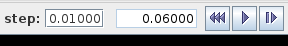
\includegraphics[]{images/playControls}
\else
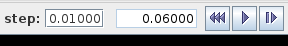
\includegraphics[width=2.5in]{images/playControls}
\fi
\end{center}
\caption{The ArtiSynth play controls. From left to right: step size
control, current simulation time, and the reset, play/pause, and
single-step buttons.}%
\label{PlayControlsFig}
\end{figure}

An extended set of play controls is available in the ArtiSynth
timeline (Section \ref{TimelinePlayControls}).

\section{The Viewer}

The viewer provides interactive graphical rendering of the ArtiSynth
model and permits selection of its components. A viewer is integrated
into the ArtiSynth main frame; additional viewers can be created
if necessary.

\subsection{Viewer Toolbar}

Each viewer is provided with a toolbar (Figure \ref{ViewerToolbarFig}) equipped
with icons for controlling the viewpoint (Section \ref{ViewpointControlSec}) and
clipping planes (Section \ref{ClippingPlanesSec}). The toolbar for the main viewer
appears vertically at the lower left of the main frame, while toolbars
for additional viewers appear horizontally at the top.  Each is an
instance of Java's {\tt JToolBar}, and so can be moved and docked
accordingly.

\begin{figure}
\begin{center}
\iflatexml
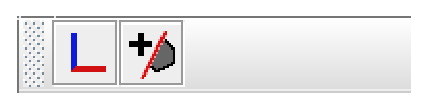
\includegraphics[]{images/viewerToolbar}
\else
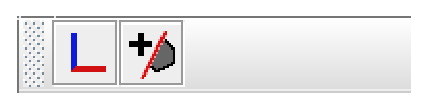
\includegraphics[width=2.5in]{images/viewerToolbar}
\fi
\end{center}
\caption{The viewer toolbar.}%
\label{ViewerToolbarFig}
\end{figure}

\subsection{Viewpoint Control}
\label{ViewpointControlSec}

The view point can be controlled interactively by dragging the middle
mouse button:

\begin{description}

\item[MIDDLE mouse] \mbox{}

Rotates the view point about the center of the frustum.

\item[SHIFT MIDDLE mouse] \mbox{}

Translates the view point in a plane perpendicular to the
line of sight.

\item[CTRL MIDDLE mouse {\it or} mouse WHEEL] \mbox{}

Zooms in or out by moving the viewpoint along the line of sight. Rotate 
wheel forward or drag mouse forward with CTRL and middle mouse button 
pressed to zoom in. Rotate or drag backwards to zoom out.

\end{description}

\label{axisAlignedViewpointsSec}
Predetermined viewpoints can also be selected using the {\it align axis}
button located on the viewer control bar.  Clicking on this
button produces an icon menu showing six different axis-aligned views.
Each view is indicated by the two axes perpendicular to the line
of sight, with the X, Y, and Z axes illustrated
by red, green, and blue lines respectively:

%\begin{description}

\begin{tabular}{l l l}
\iflatexml

\includegraphics[]{images/alignFront}
\else

\includegraphics[width=.33in]{images/alignFront}
\fi
& Front: & Z axis up, X axis to the right.\\
\iflatexml

\includegraphics[]{images/alignBack} 
\else

\includegraphics[width=.33in]{images/alignBack} 
\fi
& Back: & Z axis up, X axis to the left.\\
\iflatexml
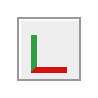
\includegraphics[]{images/alignTop} 
\else
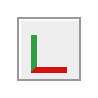
\includegraphics[width=.33in]{images/alignTop} 
\fi
& Top: & Y axis up, X axis to the right.\\
\iflatexml
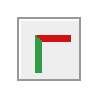
\includegraphics[]{images/alignBottom} 
\else
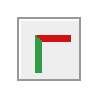
\includegraphics[width=.33in]{images/alignBottom} 
\fi
& Bottom: & Y axis down, X axis to the right.\\
\iflatexml

\includegraphics[]{images/alignLeft} 
\else

\includegraphics[width=.33in]{images/alignLeft} 
\fi
& Left: & Z axis up, y axis to the right.\\
\iflatexml

\includegraphics[]{images/alignRight} 
\else

\includegraphics[width=.33in]{images/alignRight} 
\fi
& Right: & Z axis up, y axis to the left.
\end{tabular}
%\end{description}

The align axis button itself displays the most recently selected axis-aligned
view.

\subsection{Adding Additional Viewers}

Additional viewers can be created by selecting {\sf View > New viewer}
from the main menu. Each viewer provides independent viewing and
selection control for the current model.

\begin{sideblock}
We are considering adding an option whereby the main viewer can
be split into four independent viewing panels, providing
orthogonal projections of the front, side, and top, along
with a general perspective projection. This arrangement is common
in CAD and geometric modeling applications.
\end{sideblock}

\subsection{Orthographic vs. Perspective Projection}

The user can toggle between orthographic and perspective projection by
selecting {\sf View > Orthographic view} or {\sf View > Perspective view}
from the main menu. Toggling can also be achieved using the '{\tt o}' key
within the viewer.

\subsection{Viewer Grid}
\label{ViewerGrid}

Hitting the '{\tt g}' key within the viewer enables or disables a grid
(Figure \ref{viewerGridFig}). Grid cells are square and appear in two
resolutions, with {\it major cells} subdivided into a number of {\it
minor cells}. Major cells are typically rendered more brightly than
minor cells. By default, the grid computes the cell sizes
automatically based on the current viewer zoom-level. However, it is
possible to set an explicit grid resolution (see
\ref{GridUnitsAndProperties}).

The grid is located in the plane perpendicular to the line of sight of
the most recently selected axis-aligned view. To change the grid
plane, select a new axis aligned viewpoint (Section
\ref{axisAlignedViewpointsSec}).

\begin{figure}
\begin{center}
\iflatexml
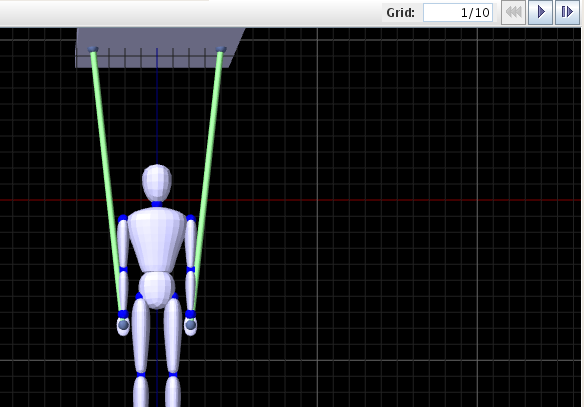
\includegraphics[]{images/viewerGrid}
\else
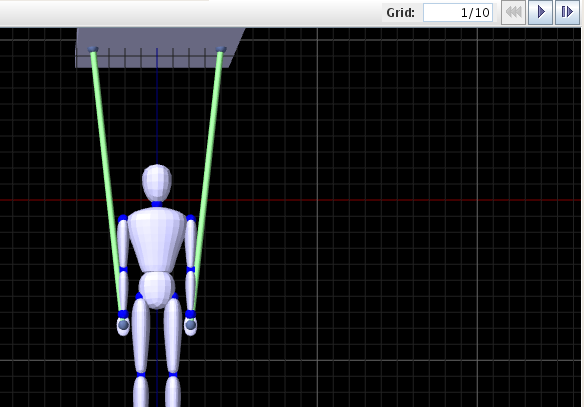
\includegraphics[width=0.66\textwidth]{images/viewerGrid}
\fi
\end{center}
\caption{Viewer showing the grid.}%
\label{viewerGridFig}
\end{figure}

\subsubsection{Grid units and properties}
\label{GridUnitsAndProperties}

When the grid is enabled, a box labeled {\sf Grid:} appears in the
toolbar on top of the main ArtiSynth frame which gives the current
resolution of the grid, displayed as {\tt S/N}, where {\tt S} is the
size of each major grid cell and {\tt N} is the number of subdivisions
per cell. If there are no subdivisions, then the {\tt /N} is omitted.
For example, in Figure \ref{viewerGridFig}, this appears as {\tt Grid:
1/10}, which means that the major grid cells have a size of 1.0 and
are each divided into 10 subdivisions. The numeric value of the ratio
{\tt S/N} gives the minor cell size.

By default, the grid automatically resizes itself to the current
viewer zoom level, choosing well-rounded numbers for the grid cell
size. Auto-sizing can be enabled or disabled by right clicking on the
{\tt Grid:} label and choosing {\sf Turn auto-sizing on} or {\sf Turn
auto-sizing off}, as appropriate. The user can also specify an
explicit value for the grid resolution by entering the desired {\tt
S/N} value (or just an {\tt S} value) into the {\tt Grid:} box.
Specifying an explicit value will disable auto-sizing, unless {\tt S}
is specified as 0 or the special value {\tt *} is entered, both of
which will renable auto-sizing.

The grid has a number of properties that can be set by right clicking
on the {\tt Grid:} label and choosing {\sf Set properties}. This will
bring up a property dialog. Properties that can be set include the
minimum size, the minimum minor cell size in pixels (when
auto-sizing), colors for the major and minor cell divisions, and
colors for the horizontal (x) and vertical (y) axes. Some of these
colors are optional and can set set to {\tt null}, in which case a
default color is computed or the associated feature is not displayed.

\subsection{Clipping Planes}
\label{ClippingPlanesSec}

The user can add clipping planes to the viewer. These are useful for
restricting what is rendered and allowing a better view of interior
structures, as shown in (Figure \ref{clipPlaneFig}).

\begin{figure}
\begin{center}
\iflatexml

\includegraphics[]{images/clipPlane}
\else

\includegraphics[width=0.66\textwidth]{images/clipPlane}
\fi
\end{center}
\caption{Clipping plane showing interior of tongue model (left), disabled (center), and in slice mode (right).}%
\label{clipPlaneFig}
\end{figure}

\subsubsection{Adding and removing}

To add a clipping plane, left click on the {\sf add clip plane}
button 
\includegraphics[width=.25in]{images/addClipPlane} located on the
viewer toolbar. This will create a clipping plane located in the plane
perpendicular to the current line of sight.

It will also add to the viewer toolbar a {\sf clip plane} icon

\includegraphics[width=.25in]{images/clipPlaneIcon} for controlling the
clipping plane.  Right clicking on this icon will bring up an option
menu.

To delete a clipping plane, right click on its icon and
select {\sf Delete}.

\subsubsection{Moving}

A clip plane is associated with a coordinate system and can be moved
and/or rotated by dragging on the trans-rotate transformer located at
its coordinate system origin. The clip region is the half space lying
in the direction of the +z axis.

The transformer itself can be made invisible/visible by right clicking
on the clip plane icon and selecting {\sf Hide transformer} or {\sf Show
transformer}.

\subsubsection{Offsets}

The clipping region is the half space lying in the direction of the +z
axis of the plane's local coordinate system. By default, clipping is
actually offset by a small distance along the +z axis, so that small
objects (such as points) lying in the x-y plane remain
visible. The amount of this offset is controlled by the plane's
{\sf offset} property, which is set to a nominal default value. To control
this property directly, right click on the clip plane icon and select
{\sf Set properties}. This will bring up a panel which allows the offset
to be adjusted.

\subsubsection{Enabling/disabling}

Left clicking on the clip plane icon will enable/disable
clipping. Disabling clipping allows the plane to be used as a regular
movable grid. When clipping is disabled, the icon
will change to the form
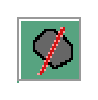
\includegraphics[width=.25in]{images/clipPlaneOffIcon}.

\subsubsection{Slicing mode}

Clipping planes can be placed in a {\it slicing mode}, whereby half-spaces
in both the positive and negative z directions are clipped. The result
is a small slice about the local x-y plane (Figure \ref{clipPlaneFig},
right). The width of this slice is controlled by the plane's {\sf offset}
property, as described above.

To enable or disable slicing, right click on the clip plane icon
and select {\sf Enable slicing} or {\sf Disable slicing}.

\subsubsection{Other features}

\begin{description}

\item[Properties]\mbox{}

Various properties associated with the plane, such as its color, line
width, cell resolution, etc., can be set explicitly by the user. To do
this, right click on the icon, select {\sf Set properties}, and edit
the resulting property panel.  Most properties are the same as those
described for the main viewer grid in \ref{GridUnitsAndProperties}.

\item[Grid visibility]\mbox{}

To make the grid invisible/visible, right click on the icon
and select {\sf Hide grid} or {\sf Show grid}.

\item[Alignment with world axes]\mbox{}

The clip plane can be aligned so that it's
normal lies along the positive or negative direction of either the x,
y, or z world axes. Right click on the icon and select the
appropriate option. Clipping is performed so that
the half-space lying in the direction of the normal is clipped.

\item[Alignment with current line of sight]\mbox{}

To align the clipping plane so that it is perpendicular to the
current line of sight, right click on the icon and select {\sf Reset}.

\end{description}

\subsection{Indicating 3D Positions with the Mouse}
\label{indicatingPositionsSec}

It is possible to use a viewer in combination with a mouse to specify the
position of a 3D point in space. This is commonly employed in the
editing operations described in Section \ref{componentEditingSec}.

To specify a point, the user left-clicks the mouse in the viewer, at
the screen postion located over the point's desired position. The 3D
position is then determined by intersecting the ray indicated by the
mouse clock with some appropriate surface or plane. Typically, a plane
perpendicular to the viewing direction and passing through the model's
center is used. Alternatively, some interactions provide a {\sf constrain
to plane} option, which causes the ray to be intersected witha viewer
clipping plane (Section \ref{ClippingPlanesSec}), providing more precise control
over the point's position. This requires that the viewer presently
contain at least one clipping plane. If more than one clipping plane
is present, the first one is used.

In other applications, the desired point may be known to lie on a 3D
surface, in which case the position is determined by intersecting the
ray with a 3D surface mesh.

\section{Component Navigation and Selection}

An ArtiSynth model is composed of a hierarchical arrangement of
model components (each of which implements the interface 
\javaclass[artisynth.core.modelbase]{ModelComponent}), 
some of which may themselves
be models. The graphical interface allows users to navigate this
hierarchy and select individual components. Selected components
can then be edited, or have specific properties modified or attached
to probes or control panels.

\subsection{The Component Hierarchy}

An example component hierarchy is shown in Figure
\ref{hierarchyFig}. At the top is a {\it root model} (class
\javaclass[artisynth.core.workspace]{RootModel}), 
in this case named {\tt Rigid Body Spring}.  The
root model in turn contains a list of models, one of which is a
mechanical model named {\tt msmod}, which here contains particles and
rigid bodies.

It is important to node that in the component hierarchy, any collection
of components is itself a component (usually an instance of
\javaclass[artisynth.core.modelbase]{ComponentList}). 
This provides automatic ``grouping'' of
components of like type, but does introduce additional levels into the
hierarchy. Hence the particle {\tt red} is a child not of {\tt msmod},
but rather the component list {\tt particles}.

\begin{figure}
\begin{center}
\iflatexml
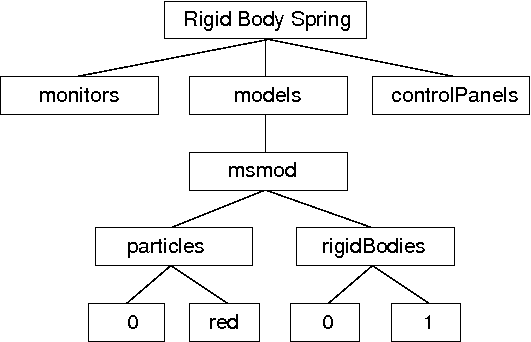
\includegraphics[]{images/hierarchy}
\else
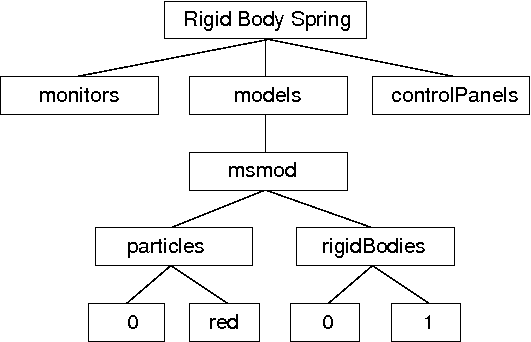
\includegraphics[width=0.66\textwidth]{images/hierarchy}
\fi
\end{center}
\caption{A sample component hierarchy.}%
\label{hierarchyFig}
\end{figure}

\subsubsection{Component names and numbers}

Model components may be assigned a string name; at the time of
this writing names may not begin with a digit, have zero length, contain
the characters '{\tt .}' or '{\tt /}', or equal the reserved word {\tt this}.
Components which do not have an assigned name are
called {\it nameless}.

All components have a {\it number}, even if they do not have a name. The
number is assigned automatically when the component is added to the
parent, and is guaranteed to be persistent until the component is
removed from the parent.

\subsubsection{Component path names}
\label{pathNamesSec}

The names and/or numbers of a component's ancestors can be used to
form a {\it component path name}. This path has a construction completely
analogous to Unix file path names, with the '{\tt /}' character acting as
a separator. Absolute paths start with '{\tt /}' and begin with the root
model. Relative paths omit the leading '{\tt /}' and can begin lower down
in the hierarchy.  The absolute path name of the {\tt red} particle in
Figure \ref{hierarchyFig} would be

\begin{verbatim}
/Rigid Body Spring/models/msmod/particles/red
\end{verbatim}

For nameless components in the path, their
numbers can be used instead:

\begin{verbatim}
 /Rigid Body Spring/models/msmod/rigidBodies/1
\end{verbatim}

Numbers can be used even for components that have names.
Hence a path name consisting only of numbers, as in

\begin{verbatim}
 /0/0/0/3/1
\end{verbatim}

is legal, although it most likely to appear only in machine-generated
output.

\subsection{Navigation Panel Selection}
\label{navPanelSec}

A navigation panel in the main ArtiSynth frame allows direct
navigation of the component hierarchy. The panel can be
open or closed by clicking on the menu bar icon 
\iflatexml

\includegraphics[]{images/navpanelIcon}.
\else

\includegraphics[width=.25in]{images/navpanelIcon}.
\fi

Figure \ref{navpanelFig} shows an navigation panel containing a superset
of the hierarchy diagrammed in Figure \ref{hierarchyFig}.

\begin{figure}
\begin{center}
\iflatexml
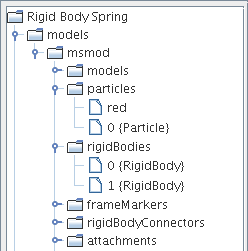
\includegraphics[]{images/navpanel}
\else
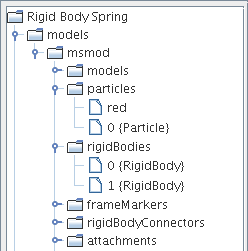
\includegraphics[width=0.30\textwidth]{images/navpanel}
\fi
\end{center}
\caption{An typical navigation panel display.}%
\label{navpanelFig}
\end{figure}

Left clicking on any component in navigation panel selects that
component. Clicking while pressing the {\tt CTRL} key
allows selection of multiple components. Clicking while
pressing the {\tt SHIFT} key allows selection of a range of components.

\subsubsection{Large numbers of nameless components}

In some cases, such as finite element models, the number of child
components can be very large (on the order of thousands). In order to
keep the navigation panel size manageable, the number of nameless
children displayed is limited to a set number (currently 100).  If the
number of nameless children exceeds this number, the display will be
augmented with an expand icon {\tt >>>}. Clicking on this will expand the
display to include all nameless components, and the expand icon will
be replaced by a contract icon {\tt <<<}. Clicking on the contract icon
will cause the extra nameless components to be hidden again.
This is illustrated in Figure \ref{navpanelExpandContractFig}.

\begin{figure}
\begin{center}
\iflatexml
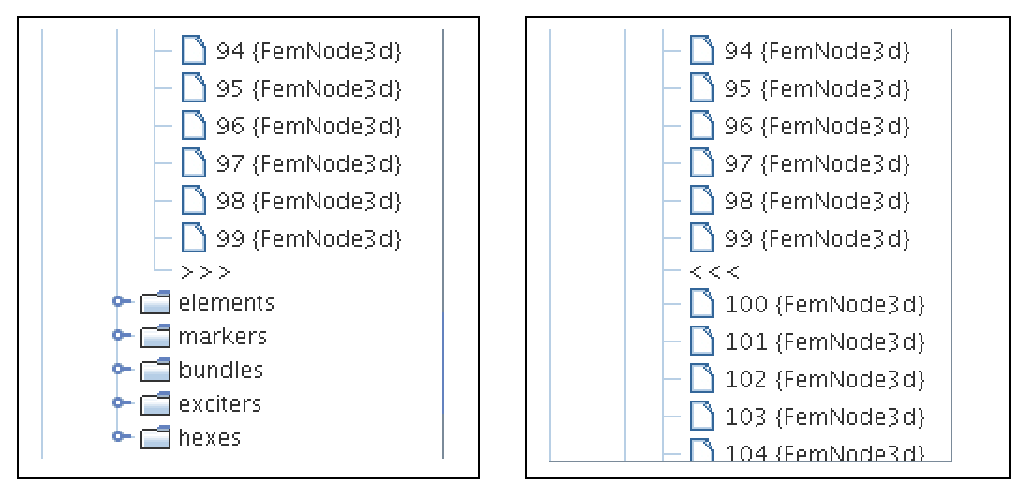
\includegraphics[]{images/navpanelContractExpand}
\else
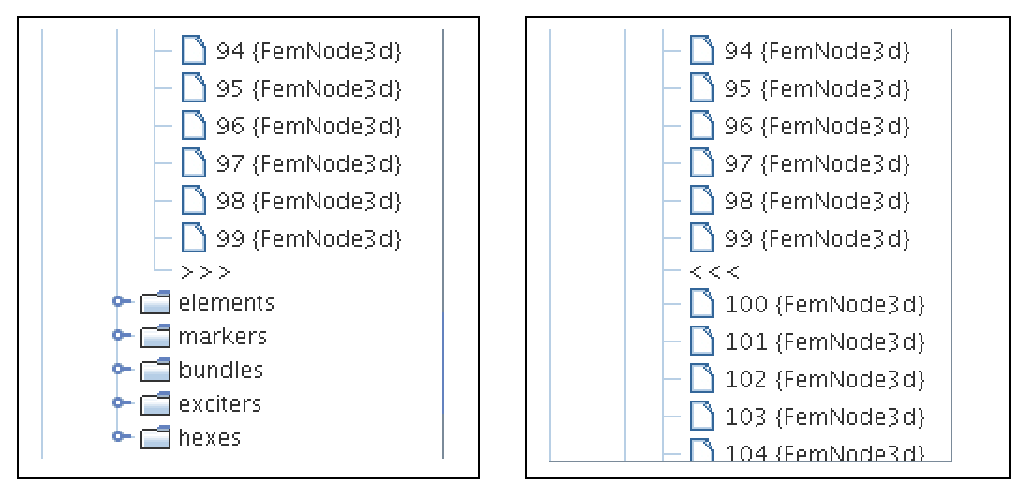
\includegraphics[width=0.66\textwidth]{images/navpanelContractExpand}
\fi
\end{center}
\caption{Expansion of nameless components in the navigation panel.}%
\label{navpanelExpandContractFig}
\end{figure}

\subsection{Viewer Selection}
\label{viewerSelectionSec}

Components that are rendered in the viewer can generally be selected
by left clicking on them (the exception would be for a few renderable
components that do not support selection). Holding the {\tt CTRL} key
allows the selection of multiple components.

\subsubsection{Box selection}

Left-clicking and dragging in the viewer allows the selection of all
components drawn within the resulting drag box. Because this often
results in the selection of more components than desired, it may be
useful to employ a selection filter (Section
\ref{selectionFiltersSec}).

\subsubsection{Selection filtering}
\label{selectionFiltersSec}

It is possible to limit viewer selection to components of a specific
type. This can be done using the selection filter widget at the bottom
left of the main ArtiSynth frame Figure \ref{selectionFilterWidgetFig}.

\begin{figure}
\begin{center}
\iflatexml
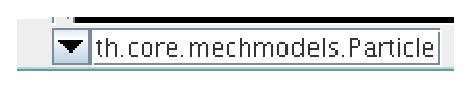
\includegraphics[]{images/selectionFilterWidget}
\else
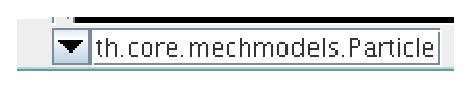
\includegraphics[width=0.40\textwidth]{images/selectionFilterWidget}
\fi
\end{center}
\caption{The selection filter widget.}%
\label{selectionFilterWidgetFig}
\end{figure}

To enable filtering, type into the widget text box the class name of
the component type you wish to restrict filtering to. It is generally
only necessary to enter the leaf name of the class (e.g., {\tt Particle}
or {\tt AxialSpring}), and the system will then find the full
class name by searching the ArtiSynth class path.

Once filtering is enabled, only components which are instances
(including subclasses) of the specified type will be selectable.

Previously selected filters can be recalled using a history
list accessible using the leftmost arrow button on the
selection widget.

To remove selection filtering, enter the special filter {\tt *}, either by
typing this in the text box, or using the history list.

\subsection{Selection Display}
\label{selectionDisplaySec}

The selection display Figure \ref{selectionDisplayWidgetFig} at the bottom of the
main ArtiSynth frame shows the full path name of the last component
added to the selection list. This is useful for identifying components
in detail.

If no components are selected, then the selection display is blank.

\begin{figure}
\begin{center}
\iflatexml
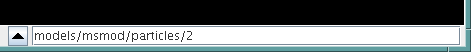
\includegraphics[]{images/selectionDisplay}
\else
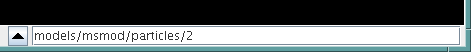
\includegraphics[width=0.50\textwidth]{images/selectionDisplay}
\fi
\end{center}
\caption{The selection display widget.}%
\label{selectionDisplayWidgetFig}
\end{figure}

The selection display is useful for disambiguating situations where it
is not clear what component we have actually selected in the viewer.
For example, FEM models keep their surface mesh contained within a
descendant component. Selecting the surface mesh will cause this
container component to be selected and highlighted, making it {\it
appear} as though the FEM model itself is selected rather than the
container. Checking the selection display makes it clear
what component has actually been selected. If desired,
one can easily navigate to one of the ancestor components
using parent selection, as described in the next section.

\subsection{Selecting Parent and Ancestor Components}
\label{selectingAncestorsSec}

Sometimes, when you select a component, you actually want to select
one of it's ancestor components. 

There are several ways to do this:

\begin{enumerate}

\item Hit the escape ({\sf ESC}) key within the viewer window. This
will select the parent of the currently selected component. Hitting
escape repeatedly is a fast way to proceed up the component hierarchy.

\item Click on the ``up'' arrow located at the left of the selection
display (Figure \ref{selectionDisplayWidgetFig}). This will also
select the parent of the currently selected component.

\end{enumerate}

Parent selection is particularly useful in the commonly occurring
situation where a composite component is not rendered and therefore
not selectable in the viewer. For instance, suppose we wish to select
a FEM model. One can select any renderable descendent of the model,
such as a node, element, or its surface mesh (if displayed), and then
use repeated parent selection until the model itself is selected.

\subsection{Highlighting Selected Components}

Selected components are rendered in the viewer using a special
selection color (yellow at the time of this writing). It is important
to note that descendents of a selected component are {\bf not} presently
rendered in any special way. For instance, if an FEM is selected, it's
nodes and elements will be rendered normally. 

While this has the potential to be confusing, we have not yet found
this to be problematic, as the navigation panel and selection display
provide alternative indicators as to what is currently selected.

\section{Geometric Manipulation}

It is possible to modify component locations, orientations, and
geometry using the transformation tools located at the left side of
the main ArtiSynth frame.  Tools will only transform those {\it
transformable} components which implement the
\javaclass[artisynth.core.util]{TransformableGeometry} interface. The
behavior may also vary depending on whether or not simulation is in
progress.

\subsection{Dragger Fixtures}
\label{draggerFixturesSec}

The transformation tools employ the dragger fixtures shown
in Figure \ref{transformToolsFig}, which allow 3D geometrical
transformations to be performed within the viewer.

\begin{figure}
\begin{center}
\iflatexml
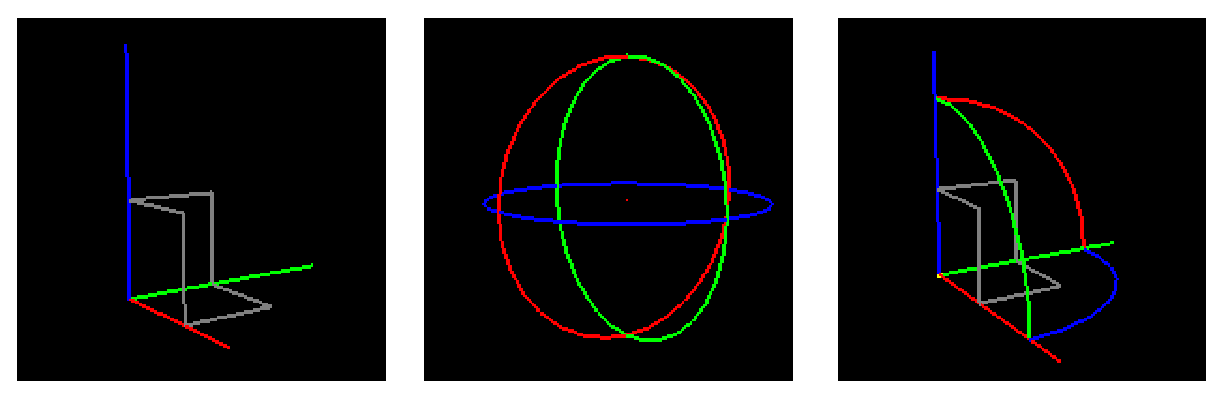
\includegraphics[]{images/transformTools}
\else
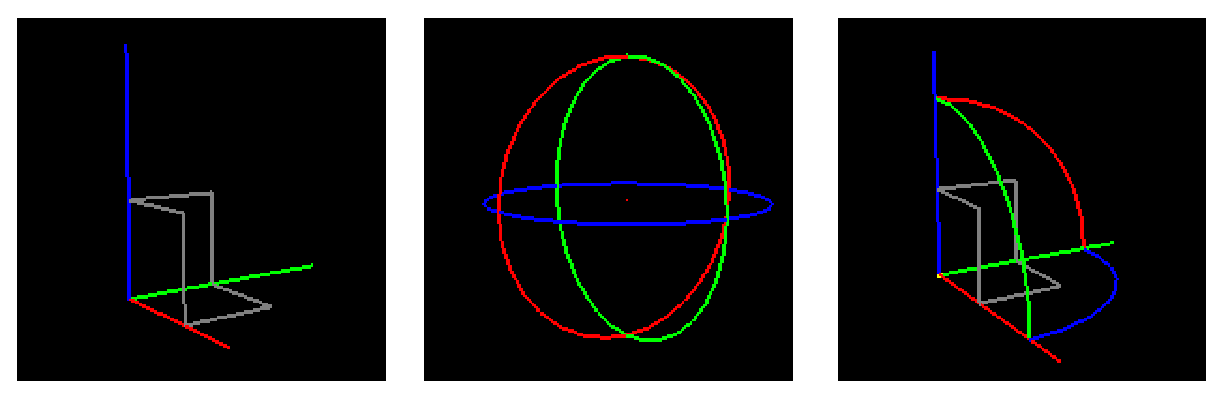
\includegraphics[width=0.80\textwidth]{images/transformTools}
\fi
\end{center}
\caption{Dragger fixtures: translator, rotator, and transrotator.}%
\label{transformToolsFig}
\end{figure}

\begin{description}

\item[Translator]\mbox{}

Effects a translation. The x, y, and z axes are
indicated by red, green, and blue lines. Dragging any line causes
a one-dimensional motion along the associated axis. Dragging one
of the boxes causes a two-dimensional motion in the associated plane.

\item[Rotator]\mbox{}

Effectors a rotation. Rotation about the
x, y, and z axes is indicated by red, green, and blue circles.
Selecting and dragging along one of these circles produces
a rotation about the corresponding axis.

\item[TransRotator]\mbox{}

Combines the translator and rotator into a single tool. One difference
is that the axes of the transRotator move with any rotation,
and so operations are done with respect to the transRotator coordinate frame
at the beginning of the drag.

\end{description}

\subsection{Manipulation Tools}
\label{ManipulationToolsSec}

A number of manipulation tools use the dragger fixtures described
above to translate, rotate, and scale components. Once a tool is
activated, then selecting one or more transformable components will
cause the corresponding dragger fixture to appear in the viewer at the
components' location. If a single component is selected and 
that component is 
associated with a coordinate frame (by implementing the
\javaclass[artisynth.core.modelbase]{HasCoordinateFrame} interface), 
then the dragger's initial position
and orientation are aligned with this coordinate frame.
Otherwise, the dragger is initially placed at the center of the
components' bounding box and its orientation is aligned to world
coordinates.

To request that a dragger's initial orientation is {\it always}
aligned with world coordinates, choose {\sf Init draggers in world
coordinates} in the ArtiSynth {\sf Settings} menu. To restore the
default behaviour, choose {\sf Init draggers in local coordinates}.

\iflatexml
% HACK: we put a '.' before the image to get LaTeXML to set it on the
% same line as the following text.
.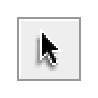
\includegraphics[]{images/selectTool}
\else
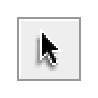
\includegraphics[width=.33in]{images/selectTool}
\fi
{\sf Selection:}\\
Normal selection mode. Turns off manipulation.

\vspace{\parskip}
\iflatexml
.
\includegraphics[]{images/translateTool}
\else

\includegraphics[width=.33in]{images/translateTool}
\fi
{\sf Translation:}\\
Translates selected components using the translator dragger.

\vspace{\parskip}
\iflatexml
.
\includegraphics[]{images/rotateTool}
\else

\includegraphics[width=.33in]{images/rotateTool}
\fi
{\sf Rotation:}\\
Rotates selected components using the rotator dragger.

\vspace{\parskip}
\iflatexml
.
\includegraphics[]{images/transRotateTool}
\else

\includegraphics[width=.33in]{images/transRotateTool}
\fi
{\sf TransRotation:}\\
Translates and rotates selected components
using the transRotate dragger. The transformation reference frame
moves with the tool.

\vspace{\parskip}
\iflatexml
.
\includegraphics[]{images/constrainedTool}
\else

\includegraphics[width=.33in]{images/constrainedTool}
\fi 
{\sf Constrained translation:}\\
Translates selected components using the translate dragger while ensuring that
they are constrained to remain on a surface mesh. Only components with
an associated surface mesh (such as FrameMarkers attached to a
RigidBody) can be manipulated this way.

\vspace{\parskip}
\iflatexml
.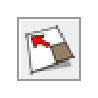
\includegraphics[]{images/scaleTool}
\else
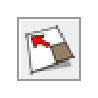
\includegraphics[width=.33in]{images/scaleTool}
\fi
{\sf Scaling:}\\
Scales selected components using the transrotator
fixture. Instead of translating, translational drag operations
scale the component along the x, y, or z axes, or in the
x-y, y-z, or z-x planes. Rotational operations, if
used in conjunction with an appropriate modifier key,
can be used to change the orientation of the scaling axes,
as described in \ref{ChangingManipulatorPose}.

\vspace{\parskip}
\iflatexml
.
\includegraphics[]{images/pullTool}
\else
\includegraphics[width=.33in]{images/pullTool}
\fi
{\sf Pulling:}\\
Pulls on points and rigid bodies using a spring-like force
when simulation is running. See Section \ref{PullManipulationSec}.

%\end{description}

\subsubsection{Constrained manipulation}

Pressing the {\tt SHIFT} modifier key causes drag operations to be
constrained to discrete step sizes. Rotation operations are
constrained to intervals of five degrees, while translation operations
are constrained to either the grid spacing (if a grid is selected, see
\ref{ViewerGrid}), or to a suitable well-rounded number depending on
the viewer's zoom level.

\subsubsection{Changing manipulator position and orientation}
\label{ChangingManipulatorPose}

Pressing the {\tt CTRL} modifier key (or the {\tt ALT} key on some
systems) causes the dragger fixture to move independently of the
selected objects. This allows its position and orientation relative to
the selected objects to be changed. This is particularly useful for
changing the orientation of the scaling directions in the scaling
tool.

\subsection{Pull Manipulation}
\label{PullManipulationSec}

\begin{figure}
\begin{center}
\iflatexml
\includegraphics[]{images/pullManipulation}
\else
\includegraphics[width=0.6\textwidth]{images/pullManipulation}
\fi
\end{center}
\caption{Applying pull manipulation (blue arrow) to a rigid body 
attached to a multi-point spring.}%
\label{PullManipulationFig}
\end{figure}

A "pull" manipulator allows a user to interactively apply a
spring-like force to either a point or rigid body by clicking on it
and then dragging (Figure \ref{PullManipulationFig}). To enable pull
manipulation, select the {\it pulling} tool (Section
\ref{ManipulationToolsSec}).

Pull manipulation is only effective when simulation is running.  It
works by adding a special {\tt PullController} to the current root
model. When attached to the root model, the controller attempts to
estimate an appropriate spring stiffness based on the overall mass and
dimensions of the first underlying {\tt MechModel}.

If necessary, the stiffness setting can also be adjusted manually by
selecting {\sf PullController > properties} in the {\sf Settings}
menu.  Render properties for the pull controller can be set from this
menu also.

\section{Editing Properties}

Most ArtiSynth model components have properties which can be 
changed onscreen through the graphical interface. Properties
include a diverse set of attributes ranging from stiffness and
damping for AxialSprings, position and velocity for particles and
rigid bodies, or whether or not a component is dynamic.

The underlying software architecture of the property interface is 
described in the 
\href{../maspack/maspack.html#Properties}{maspack documentation}.

\subsection{Property Panels}
\label{propertyPanelsSec}

To edit properties for a set of components, select the components in
question, then right click in either the viewer or the navigation
panel, and select {\sf Edit properties}. This will create a {\it property
panel} for all properties which are common to the selected components.
All typical property panel is shown in Figure \ref{propertyPanelFig}.

Property panels are initialized with the current values of the selected
components, providing a view of the current property state. A blank
property value will be displayed when more than one component is selected and 
the corresponding property value differs across components.

Some properties are {\it read only}. In this case, the corresponding
widget in the property panel will display the value but will be
disabled.

\begin{figure}
\begin{center}
\iflatexml
\includegraphics[]{images/propertyPanel}
\else
\includegraphics[width=0.40\textwidth]{images/propertyPanel}
\fi
\end{center}
\caption{A typical property panel.}%
\label{propertyPanelFig}
\end{figure}

Property panels are non-modal and persistent. 
They can be deleted by
closing them or clicking the {\sf OK} button. Clicking the {\sf Cancel} button
will cause the properties to be reset to their values at the time to
panel was created.

Normally, a property panel will refresh its widget values whenever the
model view is rerendered. In particular, this will happen repeatedly
while simulation is running. To disable the automatic refresh, click
the {\sf live updating} button 
\iflatexml
\includegraphics{images/liveUpdateIcon}
\else
\includegraphics[width=.25in]{images/liveUpdateIcon}
\fi
at the lower
left of the panel.

\subsubsection{Inheritable properties}

Some properties are inheritable. The value of an inheritable property
can be {\it explicitly} set or it can be inherited.  If inherited, then it
inherits its value from ancestor components further up the hierarchy.
More specifically, if a property's value is inherited, then the value
is obtained from the nearest ancestor in which the same property
exists and is explicitly set.  If no such ancestor exists, then the
property is set to a default value.

The inherited/explicit status of an inheritable property is controlled
by an additional button placed at the left of the property widget
(Figure \ref{inheritedButtonFig}).  Clicking this button toggles the
inherited/explicit status.  If set to inherited, then the property's
value is determined from the hierarchy and the updated value is placed
in the widget.  Setting the value in the widget itself will cause the
inheritable status to be set to explicit, and the value of inherited
instances of the same property in descendent nodes will be updated
accordingly.

\begin{figure}
\begin{center}
\iflatexml
\includegraphics[]{images/inheritedButton}
\else
\includegraphics[width=0.80\textwidth]{images/inheritedButton}
\fi
\end{center}
\caption{Property panel showing YoungsModulus as inherited (left) and 
explicitly set (right).}%
\label{inheritedButtonFig}
\end{figure}

\subsection{Render Properties}

Render properties are associated with any component that is
renderable. They are defined in the class 
\javaclass[maspack.render]{RenderProps}. 
Because of their complexity, they are adjusted
through a separate panel from the standard property panel.

To adjust the property panel for a set of components, select the components
in question, using either the viewer window or navigation panel, and then right 
click in either the viewer or the navigation panel. Several options may appear
in the context menu:

\begin{description}

\item[Edit render props]\mbox{}

This will create a special property panel allowing the render properties for
the selected components to be set (see Section \ref{renderPropSettingsSec}).

\item[Clear render props]\mbox{}

This will actually remove the render properties
from the selected components (i.e., their render properties will be
set to {\tt null}).  Nominally, this means that the components will not be
rendered, {\it unless} their parents take responsibility for rendering
children without render properties. The latter behaviour is common for
lists of particles, springs, finite elements, etc., in order to
avoid the need for defining render properties in a large number
of objects.

\item[Set visible]\mbox{}

This option will appear if any of the selected objects are
invisible. Selecting it will set the render properties so
that all components are visible.

\item[Set invisible]\mbox{}

This option will appear if any of the selected objects are
visible. Selecting it will set the render properties so
that all components are invisible.

\end{description}

\subsubsection{Render property settings}
\label{renderPropSettingsSec}

There are a large number of render property settings. Loosely
speaking, they are divided into generic settings, along with those
related to faces, lines, and points. How these are used depends on
what is being rendered. Mesh rendering typically uses the face
settings, along with the line settings to render edges if the
{\tt drawEdges} property is set {\tt true}.  Line settings are also used for
rendering axial springs and the edges of FEM elements.  Point settings
are used for rendering any subclass of Point, including Particle and
FemNode. 

Not all render properties may appear in a render panel; usually, only
those properties relevant to the selected components will be
presented.

\begin{description}

\item[Generic properties:]
\hfil \\
\begin{description}
\item[visible:]
Whether or not the component is visible.
\item[alpha:]
The transparency for polygonal faces (range 0 to 1. Default is 1, for
opaque).
\item[shading:]
How polygons are shaded ({\tt FLAT}, {\tt GOURARD}, {\tt PHONG}).
\item[shininess:]
Shininess parameter for polygons (range 0 to 32).
\end{description}

\item[Face related properties:]
\hfil \\
\begin{description}
\item[faceStyle:]
Which polygonal faces are drawn ({\tt FRONT}, {\tt BACK},
{\tt FRONT\_AND\_BACK}, {\tt NONE}).
\item[faceColor:] 
Color used for drawing faces.
\item[backColor:]
Color used for drawing backs of faces. If null, {\tt faceColor} is used.
\item[drawEdges:] 	
If true, face edgesof the polygons are drawn explicitly.
\item[textureProps:] 
Sets texture mapping properties for the face. If null, no texture
mapping is performed.
\end{description}

\item[Edge related properties:]
\hfil \\
\begin{description}
\item[edgeColor:]
The color for edges.
\item[edgeWidth:]
Edge width in pixels.
\end{description}

\item[Line related properties:]
\hfil \\
\begin{description}
\item[lineStyle:] 
How lines are drawn ({\tt CYLINDER}, {\tt LINE}, or {\tt ELLIPSOID}).
\item[lineColor:]
The color for lines.
\item[lineWidth:]
Line width in pixels when {\tt LINE} style is selected.
\item[lineRadius:]
Cylinder radius when {\tt CYLINDER} or {\tt ELLIPSOID} style is selected.
\item[lineSlices:]
Number of slices used to render {\tt CYLINDER} or {\tt ELLIPSOID} style lines.
\end{description}

\item[Point related properties:]
\hfil \\
\begin{description}
\item[pointStyle:] 
How points are drawn ({\tt SPHERE} or {\tt POINT}).
\item[pointColor:] 
The color for points.
\item[pointSize:] 
Point size in pixels when {\tt POINT} style is selected.
\item[pointRadius:] 	
Sphere radius used when {\tt SPHERE} style is selected.
\item[pointSlices:] 
Number of slices used to render {\tt SPHERE} style spheres.
\end{description}

\end{description}

\section{The Timeline}
\label{TimelineSec}

The {\it timeline} is a panel that allows the user to graphically
arrange temporal sequences of probes and waypoints to control the
simulation.

\subsection{Basic Structure}

The basic structure of the timeline is shown in 
Figure \ref{timelineFig}.

\begin{figure}
\begin{center}
\iflatexml
\includegraphics[]{images/timeline}
\else
\includegraphics[width=.75\textwidth]{images/timeline}
\fi
\end{center}
\caption{The timeline panel, containing: (A) zoom controls, (B) play
controls, (C) save button, (D) time cursor, (E) toolbar, (F) waypoint
track, (G) input track, (H) output track.}%
\label{timelineFig}
\end{figure}

The {\it toolbar} at the top contains the following widgets:

\begin{description}

\item[Zoom controls]\mbox{}

Shrinks or expands the timescale.

\item[Play controls]\mbox{}

Starts, pauses, or resets the simulation.

\item[Save button]\mbox{}

Saves the data for all probes with attached files.

\item[Time box]\mbox{}

Shows the current simulation time.

\item[Time step box]\mbox{}

Shows the length of time associated with a ``single step'' command.

\end{description}

\subsubsection{Play controls}
\label{TimelinePlayControls}

The play controls are in turn comprised of the following buttons:

\begin{tabular}{l l l}
\iflatexml
\includegraphics{images/reset}
\else
\includegraphics[width=.33in]{images/reset}
\fi
& Reset: &
Resets the simulation to the beginning at time 0.\\
\iflatexml
\includegraphics{images/fastBackward}
\else
\includegraphics[width=.33in]{images/fastBackward}
\fi
& Rewind: &
Moves the simulation time backward to the nearest
previous waypoint (see Section \ref{waypointsSec}).\\
\iflatexml
\includegraphics{images/play}
\else
\includegraphics[width=.33in]{images/play}
\fi
& Play: &
Starts the simulation.\\
\iflatexml
\includegraphics{images/pause}
\else
\includegraphics[width=.33in]{images/pause}
\fi
& Pause: &
Takes the place of the play button and pauses the simulation.\\
\iflatexml
\includegraphics{images/singleStep}
\else
\includegraphics[width=.33in]{images/singleStep}
\fi
& Single step: &
Advances the simulation by a single step, specified in the
time step box.\\
\iflatexml
\includegraphics{images/fastForward}
\else
\includegraphics[width=.33in]{images/fastForward}
\fi
& Fast forward: &
Moves the simulation time forward to the nearest
following waypoint (see Section \ref{waypointsSec}).
\end{tabular}

%\end{description}

\subsubsection{Tracks}

The timeline proper is divided into a number of tracks. At the top is
the {\it waypoint track}, which is used to arrange waypoints and 
breakpoints. Below that are a variable number of {\it input} and
{\it output} tracks, which are used respectively for arranging {\it input
probes} and {\it output probes}.


\subsection{Waypoints and Breakpoints}
\label{waypointsSec}

\subsubsection{Waypoints}

Waypoints save the model state when the simulation passes through
them, allowing the timeline to be reset to that point (using the
fast forward/backward buttons) at a later time without having to
recompute the simulation from the beginning.

Waypoints are arranged along the waypoint track at the top of the
timeline and are indicated by a small rectangular blue box
(Figure \ref{waypointsFig}). A solid box indicates a waypoint that contains a
valid state and thus can be advanced to using the fast forward/backward
buttons.

\begin{figure}
\begin{center}
\iflatexml
\includegraphics[]{images/waypoints}
\else
\includegraphics[width=0.66\textwidth]{images/waypoints}
\fi
\end{center}
\caption{Waypoints (blue) and breakpoints (red) arranged in the waypoint track.}%
\label{waypointsFig}
\end{figure}

To add a waypoint, context click on the model track.  A popup menu will
show a number of options, including {\sf Add Waypoint Here}, which adds a
waypoint at the current location of the time cursor, and {\sf Add
Waypoint(s)}, which will bring up a dialog prompting for a specific time
to add a Waypoint. The "Add Waypoint" dialog also contains a {\sf repeat}
field, which will cause additional waypoints to be added with a spacing
indicated by the time value, and an option to create breakpoints instead
of waypoints.

Once created, waypoints can be moved by dragging them. They can also
be deleted by context clicking on them and selecting the {\sf Delete Waypoint}
option.

To delete all the waypoints, context click on the model track
and select {\sf Delete Waypoints}.

\subsubsection{Breakpoints}

Breakpoints are waypoints that also cause the simulation to stop.
They are displayed in red instead of blue.

Breakpoints can be added in the same way as waypoints, i.e., by right
clicking on the model track and selecting {\sf Add Breakpoint Here} or
{\sf Add Waypoint(s)}.

Waypoints can be converted into breakpoints (and vice versa) through
the context menu.

\subsection{Tracks and Probes}

Probes are arranged on tracks located beneath the waypoint track.  Input
probes must be placed on input tracks and output probes must be placed
on output tracks.  Furthermore, probes on the same track are not allowed
to overlap.

\begin{sideblock}
{\bf Note:}\\
In the future, additional restrictions may be placed on
what type of probe can be placed on what track.
\end{sideblock}

Probes can be moved horizontally to different times as well as vertically
onto different tracks.  They can also be stretched by dragging the edges
of the probe and cropped by holding the control key while stretching.

On the left side of the timeline is the track panel, which
contains a number of track control widgets (Figure \ref{trackPanelFig}).

\begin{figure}
\begin{center}
\iflatexml
\includegraphics[]{images/trackPanel}
\else
\includegraphics[width=0.66\textwidth]{images/trackPanel}
\fi
\end{center}
\caption{Close up of the track panel, showing: (A) track panel, (B)
expand all button, (C) mute all button, (D) expand button, (E) mute
button.}%
\label{trackPanelFig}
\end{figure}

\subsubsection{Creating, moving, and deleting tracks}

New tracks may be added by context clicking in the waypoint track and
selecting {\sf Add Input Track} or {\sf Add Output Track}. 

The vertical location of a track can be moved by left clicking on it
in the left panel and dragging it up or down to a new location.

A track can be deleted by context clicking on the track in
the track panel and selecting {\sf Delete Track}.

\subsubsection{Muting tracks}

A track can be {\it muted} or {\it unmuted} by clicking on its grey mute button
in the track panel (Figure \ref{trackPanelFig}). All probes on a muted track are
ignored during simulation.

All tracks can be muted, thus disabling all probes, by clicking
on the mute all button in the grey panel above the tracks.

\subsubsection{Expanding tracks}

A track can be {\it expanded} or {\it collapsed} by clicking on its green
expand button in the track panel (Figure \ref{trackPanelFig}). Expanding a track
creates an additional area in which the data associated with the
track's probes may be displayed (see Figure \ref{numericDisplayFig}). The way
in which this data is displayed is probe-specific. Probes containing
numeric data usually show their data graphically, as described in
Section \ref{numericProbeDisplaysSec}.

\subsubsection{Grouping tracks}

Multiple contiguous tracks can be selected by clicking on them while
holding the control key.  Furthermore, they can be {\it grouped} together
or {\it ungrouped} by selecting the appropriate option from the context
menu.  Grouped tracks can be collapsed, moved simultaneously and
muted together.

\subsection{Numeric Probe Displays}
\label{numericProbeDisplaysSec}

Data associated with numeric probes is displayed as a graph within the
display (Figure \ref{numericDisplayFig}). If the probe contains a vector with
more than one value, each entry in the vector is drawn using a
different color (up to a limit, after which colors are recycled).

\begin{figure}
\begin{center}
\iflatexml
\includegraphics[]{images/numericDisplay}
\else
\includegraphics[width=0.66\textwidth]{images/numericDisplay}
\fi
\end{center}
\caption{Expanded input and output tracks showing numeric data.}%
\label{numericDisplayFig}
\end{figure}

\subsubsection{Setting the range}

The range of the displayed data can be set by context clicking in the
display and selecting {\sf Set Display Range} . This pops up a dialog that
lets the user either set the range explicitly, or enable automatic
range computation by selecting the {\sf Auto range} box.

The range of a display can also be fit to the current data
set by context clicking in the display and selecting {\sf Fit Display Range}.

\subsubsection{Visibility control}

As mentioned above, each entry in a numeric probe's data vector is
rendered in a different color (up to a limit).  If the vector has a
large dimension (say more than three), or if there is much overlapping
of values, then the result can be difficult to visualize.

To manage this problem, numeric displays provide a {\it legend} tool that
allows the user to control the color, drawing order, and visibility
for each vector entry (Figure \ref{legendFig}).

\begin{figure}
\begin{center}
\iflatexml
\includegraphics[]{images/legend}
\else
\includegraphics[width=0.30\textwidth]{images/legend}
\fi
\end{center}
\caption{Legend tool for controlling display visibility.}%
\label{legendFig}
\end{figure}

To create the legend tool, context click in the display panel and select
{\sf Legend}. Each row in the legend tool is associated with an entry in
the data vector. The dimensions of the vectors are listed, followed by 
the color the entry is drawn in and a toggle controlling its visibility.
Entries are rendered in bottom-to-top order, so those at the top will be
most visible.

\begin{itemize}

\item To change an entry's color, click the {\sf Set} button, which
will bring up a color menu.

\item To make an entry visible or invisible, use the {\sf Visible}
toggle box.

\item To change the order in which an entry is drawn, click and drag the
entry vertically within the panel.

\end{itemize}

\subsubsection{Editing data}

Data for number input probes can be changed by adding, deleting, or
moving knot points in the display.

\begin{itemize}

\item To move a knot point, left click on the knot and drag it.

\item To add a knot point, place the mouse at the desired location
and double left-click.

\item To delete a knot point, right click on the knot and select 
{\sf Delete Data Point}.

\item To edit a knot point, right click on the knot and select 
{\sf Edit Data Point}.

\end{itemize}

All knot points can be made invisible/visible by context clicking in the 
display and selecting {\sf (In)visible Data Points}.

\subsubsection{Interpolation control}

The data between knot points in a numeric probe is interpolated.
Three types of interpolation are currently available: Step, linear,
and cubic (Figure \ref{interpolationFig}). For input probes, the interpolation
can be set by right-clicking in the display and selecting the desired
one.

\begin{figure}
\begin{center}
\iflatexml
\includegraphics[]{images/interpolation}
\else
\includegraphics[width=0.66\textwidth]{images/interpolation}
\fi
\end{center}
\caption{Linear and cubic interpolation.}%
\label{interpolationFig}
\end{figure}

\subsubsection{Large displays}

A large display for a numeric probe can be created by context clicking
on the probe icon and selecting {\sf Large Display}. This will create a
large numeric display in a separate panel, allowing more precise
inspection of data (Figure \ref{largeDisplayFig}).

\begin{figure}
\begin{center}
\iflatexml
\includegraphics[]{images/largeDisplay}
\else
\includegraphics[width=0.66\textwidth]{images/largeDisplay}
\fi
\end{center}
\caption{A large display for a numeric probe.}%
\label{largeDisplayFig}
\end{figure}

In addition to the functionality of the smaller displays, large
displays have additional buttons for controlling the domain
and range of the displayed data. These are located on the left side
of the display and include four mode control buttons:

\begin{tabular}{l l l}
\iflatexml
\includegraphics[]{images/ZoomIn}
\else
\includegraphics[height=.25in]{images/ZoomIn}
\fi
& {\sf Zoom In:} &
Enables a mode in which the user can
zoom in on the display using a drag box.\\
\iflatexml
\includegraphics[]{images/ZoomOut}
\else
\includegraphics[height=.25in]{images/ZoomOut}
\fi
& {\sf Zoom Out:} &
Enables a mode in which left clicking
in the display will cause it to zoom out.\\
\iflatexml
\includegraphics[]{images/Hand}
\else
\includegraphics[height=.25in]{images/Hand}
\fi
& {\sf Move Display:} &
Enables a mode in which a (zoomed-in) display can
be moved using the middle mouse button.\\
\iflatexml
\includegraphics[]{images/Arrow}
\else
\includegraphics[height=.25in]{images/Arrow}
\fi
& {\sf Normal:} &
Clears any mode set by the previous three buttons.\\
\multicolumn{3}{p{\textwidth}}{%
\vspace{\parskip}

There are also three buttons for controlling the
vertical display range:

\vspace{\parskip}}\\
\iflatexml
\includegraphics[]{images/UpFullArrow}
\else
\includegraphics[height=.25in]{images/UpFullArrow}
\fi
& {\sf Increase Range:} &
Increases the vertical range.\\
\iflatexml
\includegraphics[]{images/DownFullArrow}
\else
\includegraphics[height=.25in]{images/DownFullArrow}
\fi
& {\sf Decrease Range:} &
Decreases the vertical range.\\
\iflatexml
\includegraphics{images/FitRange}
\else
\includegraphics[height=.25in]{images/FitRange}
\fi
& {\sf Fit Range:} &
Fits the vertical range to the current data.
\end{tabular}

%\end{description}

On the top of the display are the fields for manually setting the displayed
range and domain.  There is once again the option to enable automatic
range computation through the {\sf Auto range} box.

\section{Visual Display}

\subsection{Point Tracing}

Tracing can be enabled for individual points within an ArtiSynth
model. This causes the point to remember the path it followed since
tracing was enabled, and to render this within the viewer as strip of
line segments.

Tracing is enabled by setting a point's {\tt tracing} property to 
{\tt true} in the point's property panel (see Section \ref{propertyPanelsSec}).
When enabled, the point keeps a list of all the positions that it has
occupied since since tracing was first enabled, and renders them as a
series of line segments in the viewer.

Disabling the tracing property causes the trace data to be discarded
and it's rendering to be removed.

When tracing is enabled, the point's render properties are expanded to
include line properties. Adjusting these allow the user to control how
the trace path is rendered. When tracing is disabled, these line
properties are removed.

Since a point's render properties are modified when tracing is enabled
or disabled, any existing open rendering property panels for the
point will no longer work correctly. Instead, the panel should be
closed and reopenned.

\subsubsection{Rendering only the trace(s)}

It may be desirable to restrict rendering to view only the traces
paths, perhaps along with a few selected model components. For
instance, this might be necessary when producing graphs for a paper.

An easy way to do this is to edit the render properties for the
desired points, and set the {\tt visible} property to be explicitly
true. Then, edit the render properties for the top-level model in the
scene, and set its {\tt visible} property to be explicitly false.
This will make invisible all model components whose {\tt visible}
property is inherited. Since the traced points were explicitly set to
be visible, they (and their traces) will remain visible. If the points
themselves are rendered as spheres, they can be made to disappear by
setting their {\tt pointStyle} property to {\tt POINT}, or by setting
their {\tt pointRadius} property to something very small.

\section{Probes}

{\it Work on this section is still in progress}

\subsection{Saving and Loading Probes and Their Data}
\label{savingAndLoadingProbesSec}

The system's current probe configuration, along with the associated
probe data, can be saved in the current {\it probe directory}. Within
this directory, the information about probes is stored in a file
called {\tt probeData.art}. Actual probe data is stored in the probe's
attached file, if one is present.  Attached files are named by the
{\tt attachedFile} property of the probe, and describe the name of
the file relative to the current probe directory.

When ArtiSynth starts up, the current probe directory defaults to the
directory {\tt probeData}, relative to the working directory from
which the application was started. In future releases, when the
ability to save and restore workspaces is implemented, the current
probe directory may instead by initialized from saved workspace data.

\subsubsection{Saving probes}

Probes can be saved using the {\tt Save probes} command from the 
{\tt File} menu. This will save the current probe configuration in the
probe directory (creating this directory if necessary). It will also
save data for individual probes in their attached files, if such files
are present. 

A probe will not always have a file associated with it. Numeric probes
will always have files associated with them; if a file is not named
explicitly, a file name will be generated automatically when the probe
is added to the system. This generated file name will be unique with
respect to all probes currently configured and all files in the
current probe directory.

\subsubsection{Saving probes in a different directory}

To save probes in a different directory, one can use the command 
{\tt Save probes in} from the {\tt File} menu. This will prompt the user
for a different directory, which will be created if necessary.
The new directory will persist and the current probe directory.

\subsubsection{Loading probes}

Probes can be loaded form the current probe directory using the 
{\tt Load probes} command in the {\tt File} menu. The existing probe
configuration will be cleared and the new configuration will be
obtained from the file {\tt probeData.art}, which must be present in
the directory. Probes with attached files will be initialized from the
data in those files.

\subsubsection{Loading probes from a different directory}

To load probes from a different directory, one can use the command 
{\tt Load probes from} in the {\tt File} menu. This will prompt the user
for a different directory, which must currently exist and
which must contain the file {\tt probeData.art}. The probe
configuration will then be reset from the data in this new
directory, which will persist as the new current probe directory.

\section{Adding and Editing Numeric Probes}
\label{AddingAndEditingNumericProbes:sec}

Numeric input and output probes can be interactively added to a
simulation. Output probes allow you to record a vector of values
derived from one or more model component properties.  Input probes
allow you to use a vector of input data to drive one or more model
component properties.

\subsection{Adding Output Probes}

To add a numeric output probe, go to the main
menu and choose {\sf edit > add output probe}. This will create
a numeric output probe editor, as shown in Figure \ref{OutputProbeEditorAFig}.

\begin{figure}
\begin{center}
\iflatexml
\includegraphics[]{images/outputProbeEditorA}
\else
\includegraphics[width=0.80\textwidth]{images/outputProbeEditorA}
\fi
\end{center}
\caption{Probe editor for an uninitialized numeric output probe.}%
\label{OutputProbeEditorAFig}
\end{figure}

The editor contains three main panels:

\begin{itemize}

\item A {\it property panel} at the upper left in which allows you
to add or edit the properties of model components whose values will be used in
computing the final output probe value. Each property is
associated with a component/property widget, which allows you to first
select a component and then choose one of its properties.

\item A {\it formula panel} at the the upper right which allows
you to add or edit formulae which convert the values from
the properties into numeric values for the output probe.

\item A {\it probe property panel} at the bottom which allows properties of
the probe itself to be set.

\end{itemize}

\subsubsection{Creating a simple probe}
\label{simpleOutputProbeSec}

Creating an output probe that simply records the value of a single
numeric property is fairly easy. Starting with the output
probe editor in Figure \ref{OutputProbeEditorAFig}:

\begin{enumerate}

\item Select a component, either externally through the navigation panel
(Section \ref{navPanelSec}), the viewer 
(Section \ref{viewerSelectionSec}), or the selection
display (Section \ref{selectionDisplaySec}), or by entering its path name into the
component/property widget. Once a component is selected,
the left-most ``up'' arrow can be used to select that
component's parent.

\item Select a property for the component from the property
selection box at the right of the component/property widget.

\item Adjust any required properties for the probe itself 
(Section \ref{settingProbePropertiesSec}).

\item Click {\sf Done}.

\end{enumerate}

\subsubsection{General output probes}

In general, output probes define a general map from the numeric values
of n model component properties to a generalized output vector formed by the
concatenation of m-subvectors formed by m formulae, as shown
in Figure \ref{OutputProbeMapFig}. In the simple case of 
Section \ref{simpleOutputProbeSec},
there is a single property, one sub-vector equal to the output
vector, and a formula which is just the property value itself.

\begin{figure}
\begin{center}
\iflatexml
\includegraphics[]{images/outputProbeMap}
\else
\includegraphics[width=0.66\textwidth]{images/outputProbeMap}
\fi
\end{center}
\caption{General mapping for an output probe.}%
\label{OutputProbeMapFig}
\end{figure}

Each of the n properties has a numeric value which is
represented by a variable $p_i$ and which is a vector of some dimension
(scalars being considered vectors of dimension 1). The dimension of
the $p_i$ depends on the property and is displayed to the right of the
property selection box on the component/property widget.

Each of the m formulae is an arithmetic expression, implemented in
Jython, which may involve one or more of the variables $p_i$. The output
from each formula is itself a vector of dimension $d_j$, which is
displayed at the right of each formula panel. The simplest formula is
just a single variable $p_i$, in which case $d_j$ equals the dimension of
$p_i$. The concatenation of all the output vectors from all the formulae
produces the output vector associated with the probe, which has a
dimension $\sum_m d_j$.

\subsubsection{Using the probe editor}

What the probe editor allows you to do is create the above mentioned
map by selecting the properties of model components, assigning
variable names to them, and creating formulae using these
variables. When all the selected components form a coherent mapping,
the {\sf Done} button will be enabled and the probe can be completed. When
one or more parts of the mapping is unspecified or incomplete, the
associated widgets will be highlighted and the {\sf Done} button will be
disabled.

Extra properties can be added by requesting additional
component/property widgets using the "{\tt +}" button
in the property panel. Similarly,
extra formulae can be requested using
the add button in the formula panel.

Properties and formulas can also be deleted; simply right
click on the associated widget and choose {\sf delete}.

Property variable names appear in a box at the left of the
component/property widget. Variable names can be changed by editing
this box. Name changes will be propagated into the formulae.

In order to streamline the probe creation process, the editor will try
to guess certain desired actions.  In particular, when the user
chooses a property with a given component/property widget for the
first time, the editor assigns a variable name to that property and
creates a formula panel containing that variable. The variable name
and formula panel can be changed if necessary.

\begin{sideblock}
{\bf Note:}\\ 
The selection manager is connected to at most one
component/property widget at a time. The component field for this
widget is indicated with a blue border; external selections will
affect only that widget. Left clicking on a component/property widget
will cause it to be connected to the selection manager.
\end{sideblock}

\subsection{Adding Input Probes}

To add a numeric input probe, go to the main
menu and choose {\sf edit > add input probe}. This will create
a numeric input probe editor, as shown in Figure \ref{InputProbeEditorAFig}.

\begin{figure}
\begin{center}
\iflatexml
\includegraphics[]{images/inputProbeEditorA}
\else
\includegraphics[width=0.80\textwidth]{images/inputProbeEditorA}
\fi
\end{center}
\caption{Probe editor for an uninitialized numeric input probe.}%
\label{InputProbeEditorAFig}
\end{figure}

The editor contains three main panels:

\begin{itemize}

\item An {\it input panel} at the upper left which allows you
to add or edit input variables. Each of these variables represents
a sub-vector of the probe's numeric input vector.

\item A {\it formula/property panel} at the the upper right which allows you
to add or edit numeric properties (using component/property widgets),
along with formulae to determine values for these properties based on
the input variables.

\item A {\it probe property panel} at the bottom which allows properties of
the probe itself to be set.

\end{itemize}

\subsubsection{Creating a simple probe}
\label{simpleInputProbeSec}

Creating an input probe that simply sets a single numeric
property from the probe's input vector is fairly easy, and
is exactly analogous to creating a simple output probe
(Section \ref{simpleOutputProbeSec}). Starting with
the input probe editor in Figure \ref{InputProbeEditorAFig}:

\begin{enumerate}

\item Select a component, either externally, or using the
component/property widget.

\item Select a property for the component from the property
selection box at the right of the component/property widget.

\item Adjust any required properties for the probe itself 
(Section \ref{settingProbePropertiesSec}).

\item Click {\sf Done}.

\end{enumerate}

\subsubsection{General input probes}

In general, input probes define a general map from the probe's
input vector (which is subdivided into n input variables
of dimension $d_i$) to the values of m properties, where each
value is determined by an independent formula based
on the input variables (Figure \ref{InputProbeMapFig}).
In the simple case of Section \ref{simpleInputProbeSec},
there is one input variable which equals the input vector,
and it drives a single property using a formula which is
just the value of the input vector.

\begin{figure}
\begin{center}
\iflatexml
\includegraphics[]{images/inputProbeMap}
\else
\includegraphics[width=0.66\textwidth]{images/inputProbeMap}
\fi
\end{center}
\caption{General mapping for an input probe.}%
\label{InputProbeMapFig}
\end{figure}

Each input variable is a vector of dimension $d_i$ (scalars being
considered vectors of dimension 1), and the sum of all the $d_i$ equals
the dimension of the input vector.

Each of the formulae controlling the properties is an arithmetic
expression, implemented in Jython, which may involve one or more of
the input variables $p_i$. The output from each formula is itself a vector
whose dimension must match the associated numeric property.
The simplest formula is just a single variable $p_i$, in which
case its dimension equals the dimension of $p_i$.

\subsubsection{Using the probe editor}

The probe editor allows you to create the above mentioned
map by creating input variables, selecting properties,
and creating formulae to drive these properties. When all the
selected components form a coherent mapping, the {\sf Done} button will be
enabled and the probe can be completed. When one or more parts of the
mapping is unspecified or incomplete, the associated widgets will be
highlighted and the {\sf Done} button will be disabled.

Extra properties can be added by requesting additional
component/property widgets using the "{\tt +}" button in the
formula/property panel. Similarly, extra input variables can be
requested using the add button in the formula panel.

Properties and input variables can also be deleted; simply right
click on the associated widget and choose {\sf delete}.

Each input variable is associated with a widget containing two text
fields, the left one defining the variable's name and the right one
its dimension.  The name or dimension can be changed by editing these
fields. Changes will be propagated into the formulae; formulae that
are found to be incompatible with the changes will be cleared.

In order to streamline the probe creation process, the editor will try
to guess certain desired actions.  In particular, when the user
chooses a property with a given component/property widget for the
first time, the editor creates an input variable whose dimension
matches the property, and a simple formula consisting solely
of the input variable. The input variable and formula can be changed if
necessary.

\begin{sideblock}
{\bf Note:}\\
The selection manager is connected to at most one
component/property widget at a time. The component field for this
widget is indicated with a blue border; external selections will
affect only that widget. Left clicking on a component property widget
will cause it to be connected to the selection manager.
\end{sideblock}

\subsection{Setting Probe Properties}
\label{settingProbePropertiesSec}

The lower part of the probe editor contains a set of fields for
editing various probe properties.

\begin{description}

\item[name]\mbox{}

The name of the of the probe.

\item[start time]\mbox{}

Start time for the probe, in seconds.

\item[stop time]\mbox{}

Stop time for the probe, in seconds.

\item[scale]\mbox{}

Specifies the scale $s$ for this probe, which relates the internal probe 
time $t_p$ to the external simulation (or timeline) 
time $t$. If $t_\text{start}$ is the time
at which the probe starts on the timeline, then $t = t_p s + t_\text{start}$.

\item[attached file]\mbox{}

Names the {\it attached file} for this probe, used for
storing the probe's date. See Section \ref{savingAndLoadingProbesSec}.

\item[display range]\mbox{}

Minimum and maximum range values used for the graphical display
of the probe's data. If these values are left blank, then
the range is computed automatically.

\item[update interval]\mbox{}

(Output probes only). A time interval, in seconds, specifying
how often data should be output to the probe. 

\end{description}

\section{Making Movies}

ArtiSynth includes a panel to aid in capturing simulations as
movies. This panel is opened from the main viewer window by navigating
through {\sf View > Show movie panel}. When capturing a movie, pictures are
saved to {\tt ARTISYNTH\_HOME/tmp} periodically as frameXXXXX.ext, where
XXXXX represents the sequential number of the frame (with each X
representing a digit), and the .ext represents the file extension
(determined by the {\sf Frame File} selection in the encoder panel). Because
the frame files aren't unique, recordings will overwrite frames from
prior movies, and if {\sf Remove temporary files} is selected, only the final
products are left. When the recording is stopped, these pictures are then
compressed into a movie file using either mencoder, or an internal
algorithm. The resulting movie is saved to the {\tt \$ARTISYNTH\_HOME/tmp} with
the file name specified at the bottom of the recorder panel.

\begin{figure}
\begin{center}
\iflatexml
\includegraphics[]{images/moviePanel}
\else
\includegraphics[width=0.40\textwidth]{images/moviePanel}
\fi
\end{center}
\caption{Movie options panel (recorder tab).}%
\label{movieOptionsRecorderFig}
\end{figure}

\begin{figure}
\begin{center}
\iflatexml
\includegraphics[]{images/moviePanel2}
\else
\includegraphics[width=0.40\textwidth]{images/moviePanel2}
\fi
\end{center}
\caption{Movie options panel (encoder tab).}%
\label{movieOptionsEncoderFig}
\end{figure}

\subsection{Region To Capture Options}

These options define the area of the desktop recorded. The default
capture area is the main viewer of ArtiSynth. {\sf Viewer} sets the capture
area exclusively and strictly to the main viewer, and excludes the toolbar
and window. This is useful for recording model demonstrations. The
{\sf Window} option includes the main viewer and the toolbar and window
surrounding it. The {\sf Custom} option allows the user to manually set the 
coordinates, width and height of the region to capture through the given
fields.  It also displays the capture frame, which can be stretched and 
moved to adjust what is recorded.

When the {\sf Viewer} mode is selected, there are additional options
available in the {\sf Output Size} section.  This allows you to create
higher (or lower) resolution videos, independent of the viewer's 
visible resolution.  The {\sf \# samples} specifies the size of the
multi-sample buffer, which is used for anti-aliasing.  This is the
only mode that continues to work correctly when a screen-saver
is activated.  

\subsection{Record Options}

These options determine how the movie recorder works with ArtiSynth,
and how it deals with the frame files.

\begin{description}

\item[Begin playing on start]\mbox{}

When the {\sf start} button is clicked, the simulation will begin to run.

\item[End playing on stop]\mbox{}

When the {\sf stop} button is clicked, the simulation stops running.

\item[Automatic frame capature]\mbox{}

Frames are automatically captured according to the movie's frame-rate 
while the model is run.  If this is disabled, it is up to the user
to click on the {\sf Frame} button to capture the next frame.

\item[Remove temporary files]\mbox{}

When selected, the temporary frames are deleted after the movie is made.

\item[Save first image]\mbox{}

This saves the first frame taken. These frames are useful for
representing the movie in websites.

\item[Show capture frame]\mbox{}

Opens a transparent window that reveals what will be captured. The window
is stretchable and movable when the capture option is set to {\sf Custom} and
provides a method to graphically modify the capture area's X coordinate,
Y coordinate, width, and height.

\end{description}

\subsection{Output Options}

These options control the frequency of the frames and how they are
combined into a movie.

\begin{description}

\item[Frame rate]\mbox{}

This is the number of frames recorded per second of movie.

\item[Speed]\mbox{}

This is the ratio of the movie's speed to reality's speed. While the
demo is recording, the calculations may slow down the simulation, but
the movie will not be affected.

\begin{sideblock}
{\bf Important:}\\
If the {\sf Frame Rate} or {\sf Speed} is set so that the
increments between the frames is smaller than the calculation steps
used in the, then ArtiSynth will decrease the calculation increments
in order to capture the frames, slowing the simulation.
\end{sideblock}

\item[Frame File]\mbox{}

This is the format the frames will be stored in. If the internal
method (see below) is used, then the frames must be stored as jpegs.

\item[Method]\mbox{}

This is the algorithm used to compress the temporary pictures into a movie.

\begin{itemize}

\item {\sf internal} Use ArtiSynth's built in algorithm to compress the
pictures into an animated jpeg.

\item {\sf mencoder} Use Mencoder to compress pictures into a divx movie
(can be played on MediaPlayer with a plugin).

\item {\sf mencoder\_osx} This option is specific for use on MacOS.

\item {\sf ffmpeg} Use the FFMPEG command-line utility to generate
the movie.

\item {\sf animated\_gif} Uses an algorithm built into ArtiSynth to
generate an animated gif.  By hitting the {\sf Customize Method}
button, you can set the number of times to loop (-1 for infinity)
and the frame rate (defaults to capture frame rate).

\item {\sf avconv} Uses the avconv utility that has replaced
FFMPEG on some linux systems to generate the movie.

\end{itemize}

\end{description}

The customize button right of the method box opens a window where the
specific command calling mencoder can be edited. The variables
identified with the '\$' are the input parameters for the mencoder,
and are based on information provided to the movie panel.

\begin{description}

\item[\$FMT]\mbox{}

Controls the format of the frames. Modifying this is the same as
changing {\tt Frame File}.

\item[\$OUT]\mbox{}
 
The name of the output file. Modifying this is the same as
changing the {\tt name} field.

\item[\$FPS]\mbox{}

Determines the frame rate mencorder uses when it compiles the
movie. By default, this is the same as the {\tt Frame Rate} option.

\end{description}

\subsection{Output Size Options}

These options are only used when the capture area is set to {\sf Viewer} and
control the size of the output video, allowing the contents of the viewer
to be magnified.

\begin{description}

\item[Same to original size]\mbox{}

The output video is created at the original size.

\item[Constrain proportions]\mbox{}

The output video is created with constrained proportions, such that the ratio
between height and width are maintained.

\item[Width]\mbox{}

Defines the width of the output video. 

\item[Height]\mbox{}

Defines the height of the output video. 

\item[\# samples]\mbox{}

Sets the number of samples to use for the multi-sample buffer.  This only
applies in {\sf Viewer} mode, and is used to perform anti-aliasing.

\begin{sideblock}
{\bf Note:} If your movie comes out black or only shows a section of 
the viewer correctly in {\sf Viewer} mode, then it is likely your
graphics card does not support multi-sample buffers.  On machines 
with multiple graphics cards (e.g. laptops with both discrete and
integrated graphics), make sure the java process is set to use
the discrete card.  Otherwise, set {\sf \# samples = 1} to disable
the multi-sample buffer.
\end{sideblock}

\end{description}

\section{Control Panels}

Control panels are essentially custom-built property panels that are
attached to the root model and let the user interactively set or
adjust various properties while the simulation is in progress.
Most of the panels that appear with the various ArtiSynth demos
are in fact control panels specially created for the demo in question.

The properties controlled by a control panel do not need to come from
the same object; instead, they can come from a variety of objects.
However, unlike with property panels, it is not possible (at the time
of this writing) for a control panel widget to control a property across
multiple objects.

\begin{sideblock}
The problem of controlling the same property in multiple objects
may be addressed in future by the introduction of {\it component groups}.
\end{sideblock}

\subsection{Creating Control Panels}

To create a control panel, select {\sf Edit > Add control panel} from the
ArtiSynth main menu. This will cause a blank control panel to appear.

To add a widget to this panel, right click inside the the panel and select
{\sf Add widget}. This will cause a widget creation dialog to appear,
as shown in Figure \ref{widgetCreationDialogFig}.

\begin{figure}
\begin{center}
\iflatexml
\includegraphics[]{images/widgetDialog}
\else
\includegraphics[width=0.66\textwidth]{images/widgetDialog}
\fi
\end{center}
\caption{Widget creation dialog.}%
\label{widgetCreationDialogFig}
\end{figure}

The top-most widget in this dialog is a component/property
selector. The component section is a selection display identical in
function to that described in Section \ref{selectionDisplaySec}: the path of the
most recently selected component is displayed, and its parent may be
selected by clicking on the ``up'' button at the left. If no component
is selected, you will need to select one using the navigation panel or
the viewer.  Once a component is selected, the combination box on the
right will provide a selection of properties that may be selected for
the widget. Once a property is selected, other options in the dialog
may be used to tune the appearance of the widget:

\begin{description}

\item[slider]\mbox{}

Enabled for properties with a scalar numeric value.
Setting it to true will create a widget with a slider.

\item[range]\mbox{}

Specifies the range for the slider, if one is selected.

\item[labelText]\mbox{}

The name of the widget in the panel. By default, this is the
name of the property.

\item[labelFontColor]\mbox{}

Font color for the widget name. If {\tt null}, then the default color 
is used.

\item[backgroundColor]\mbox{}

Background color for the widget. If {\tt null}, then the default 
background is used.

\end{description}

\subsubsection{Composite property widgets}

A \javaclass[maspack.properties]{CompositeProperty} is a Property which contains
sub-properties. If a composite property is selected, the control panel
will create a {\it composite property widget}, three of which are shown in
Figure \ref{compositePropWidgetsFig}.

\begin{figure}
\begin{center}
\iflatexml
\includegraphics[]{images/compositePropWidgets}
\else
\includegraphics[width=0.45\textwidth]{images/compositePropWidgets}
\fi
\end{center}
\caption{Composite property widgets.}%
\label{compositePropWidgetsFig}
\end{figure}

Clicking the {\sf set} button of a composite property widget will create
another panel presenting all the sub-properties. The composite
property widget is disabled until this panel is closed.

In some instances, a composite property can be set to {\tt null}.  In such
cases, the widget will provide an additional component, which

\begin{itemize}

\item if the current property value is {\bf not} {\tt null}, will be a 
{\sf clear} button which sets the value to {\tt null} 
(second widget, <Figure \ref{compositePropWidgetsFig}).

\item if the current property value {\bf is} {\tt null}, will be a display label
indicating this fact (third widget, <Figure \ref{compositePropWidgetsFig}).

\end{itemize}

\subsubsection{Widgets for sub-properties}

It is possible to attach widgets to the sub-properties of a 
composite property, provided that the composite property 
has a non-null value.

In particular, when a non-null composite property is selected from the
component/property widget, the user has the option of either

\begin{itemize}

\item clicking the {\sf Done} button and selecting the composite property,
which will create a composite property widget as described in the
previous section, or

\item selecting one of the composite property's sub-properties.

\end{itemize}

When a non-null composite property is selected, the property's name
will move over into the component field of the component/property
selector, and the combination box will be cleared and reset to allow
the selection of the sub-properties.

\begin{figure}
\begin{center}
\iflatexml
\includegraphics[]{images/selectingRenderVisible}
\else
\includegraphics[width=0.66\textwidth]{images/selectingRenderVisible}
\fi
\end{center}
\caption{Selecting property renderProps (top), then one of it's 
subproperties (bottom).}%
\label{selectingRenderPropsFig}
\end{figure}

For example, in Figure \ref{selectingRenderPropsFig}, we first select
{\tt renderProps}, which is a composite property of
{\tt models/msmod/particle/2}, and then (in the lower panel) select the
sub-property {\tt visible}.  When {\tt renderProps} is selected, its name is
moved to the component panel, where it appears as

\begin{verbatim}
  models/msmod/particle/2:renderProps
\end{verbatim}

\begin{sideblock}
{\bf Note:}\\ 
The '{\tt :}' character is used to separate components from
properties in component/property paths
\end{sideblock}

\subsection{Editing Control Panels}

An existing control panel can also be edited. Specifically,

\begin{itemize}

\item Individual widgets can be moved, deleted, or have their properties
set.

\item Separators can be added between widgets.

\item Global aspects of the control panel itself can be set.

\end{itemize}

To edit an individual widget, you first select it by left-clicking on
it. This will cause it to become highlighted. You can then:

\begin{itemize}

\item {\bf Move} the widget by dragging it to a different vertical location
within the panel;

\item {\bf Delete} the widget by right-clicking and choosing {\sf delete};

\item {\bf Set properties} of the widget by right-clicking and choosing
{\sf properties};

\end{itemize}

To add a separator, select a widget above where you want the
separator, right-click and choose {\sf add separator}.

To set global aspects of the control panel itself, right-click
inside the lower-most {\it option pane} (the small panel at the
bottom and that may, in some cases, contain option buttons such as {\sf Close}
or {\sf Done}), and choose from the provided menu.

\subsection{Live Updating}

By default, a control panel is set up to update the values of its
widgets every time the viewers are rerendered. This allows one to
observe property values as they evolve in time.

If you do {\it not} want live updating of property values, then you can
disable this by clicking on the {\it live update icon}
\includegraphics{images/liveUpdateIcon}, which is located in the lower left of the
option panel.

\section{Component Editing}
\label{componentEditingSec}

Component editing in ArtiSynth is driven by the current {\it selection
context}: depending on what items are currently selected, different
editing options will appear in the context menu. These options may
allow you to add, edit, or delete components.

\subsection{Generic Edit Operations}

\subsubsection{Deletion}

A set of selected components can be deleted provided that 

\begin{itemize}

\item their parent components are editable 

\item none of their ancestors are selected

\end{itemize}

If the currently selected components are deletable, then a {\sf delete}
option will appear in the context menu (obtained by right-clicking in
the viewer or navigation panel). Selecting this will delete the
components.

If the selected components are referred to by other components, then
those components will be deleted also. In this case, a dialog will be
presented to the user advising of this fact and requesting
confirmation.

\subsubsection{Duplication}

A set of selected components may be {\it duplicated} provided that

\begin{itemize}

\item their parent components are editable

\item none of their ancestors are selected

\item they implement \javaclass[artisynth.core.modelbase]{CopyableComponent}

\end{itemize}

If the currently selected components are duplicable, then a
{\sf duplicate} option will appear in the context menu. Selecting this
will enable duplication of the components: the viewer cursor will
change to cross-hairs, and the user may indicate the location for the
duplicated components by left-clicking in the viewer
(see Section \ref{indicatingPositionsSec}).  Duplication may
be canceled by right-clicking.

Sometimes, when the components to be duplicated refer to other
components, those referred components will be duplicated also.  This is
done when the referred components are required.  For example, when
duplicating an \javaclass[artisynth.core.mechmodels]{AxialSpring}, the two
points it is attached to will also be duplicated, because AxialSprings
are not permitted to exist without attached points.  Such cases are
indicated to the user, after the {\sf duplicate} option has been selected,
by expanding the current selection to include all such additional
components.

\subsubsection{Undo}

Many of the operations described here are {\it undoable}, by choosing the
{\sf Undo} option from the {\sf Edit} menu. The menu option will indicate the
name of the operation to be undone.

\subsection{Editing Panels}

Many editing operations involve the creation of {\it editing} panels (such
as Figure \ref{addFemModelPanelFig}, etc.) which persist beyond the invocation of
a context menu. Often, these panels are created {\it exclusively}, so that
only one can be in existence at once.  This is done by having the
panel acquire a lock in the ArtiSynth editing manager. The panels are
not modal, so the user can still interact with the viewer and other
GUI components, but other exclusive editing panels can not be created
until the current one is closed. This avoids problems associated with
having two ``edits'' active on a the model at once. 

If an exclusive editing panel is open, then other exclusive editing
options will still be shown in the context menu but will be disabled.

\subsection{Specifying Position, Orientation, and Scaling}
\label{positionOrientationScalingSec}

Sometimes, an editing panel will allow you to specify the translation
and rotation associated with a
\javaclass[maspack.matrix]{RigidTransform3d}. Typically, this will happen
when there is a need to specify the location of a spatial coordinate
frame, as in the example of Figure \ref{locationPanelFig}. 

\begin{figure}
\begin{center}
\iflatexml
\includegraphics[]{images/locationPanel}
\else
\includegraphics[width=0.50\textwidth]{images/locationPanel}
\fi
\end{center}
\caption{Panel for specifying the location of a coordinate frame.}%
\label{locationPanelFig}
\end{figure}

Here, the translation
and rotation correspond to the fields {\sf position} and
{\sf orientation}. The {\sf position} field is straightforward: it is just three
numbers giving the position of the coordinate frame origin with
respect to the base (usually world) coordinates. In Figure \ref{locationPanelFig},
this is the vector (1, 2, 3).

The {\sf orientation} field is more complex. It corresponds to the rotation
of the coordinate frame with respect to base coordinates, and is
represented using an {\it axis-angle} format of four numbers giving the
axis of the rotation, followed by the angle of rotation about this
axis, in degrees.  (This relies on the fact that any 3D rotation can
be specified as a single rotation about a single axis.)  Hence the
numbers

\begin{verbatim}
 0 1 0 60
\end{verbatim}

in Figure \ref{locationPanelFig} correspond to a rotation of 60 degrees about
the y axis. Alternatively, the numbers

\begin{verbatim}
 1 1 0 45
\end{verbatim}

would correspond to a rotation of 45 degrees about the axis (1, 1, 0).
(Note that the axis does not need to be a unit vector.)
Finally, no rotation, or more precisely, the {\it identity} rotation,
is usually represented as

\begin{verbatim}
 1 0 0 0
\end{verbatim}

i.e., {\it zero} rotation about the x-axis. In more general situations,
one may specify not only translation and rotation but also scaling,
corresponding to a more general
\javaclass[maspack.matrix]{AffineTransform3d}. This often occurs when
reading a mesh from a file: one may wish to apply an affine transform
to scale, rotate, and translate the mesh that is been read in.  In
such cases one will also be presented with a {\sf scale} field, which
accepts either a single number (to denote uniform scaling), or three
numbers (to denote non-uniform scaling about the x, y, and z axes).

\subsection{Editing MechModels}

A \javaclass[artisynth.core.mechmodels]{MechModel} is the central ArtiSynth
component for mechanical simulation. It contains sets of mechanical
components, including particles, rigid bodies, axial springs, rigid
body connectors, as well as sub-models including other {\tt MechModels}
and finite element (FEM) models. Most of these components can be added to a
MechModel graphically, as described below.

To add a component to a MechModel, select the MechModel and choose the
appropriate edit action shown in the context menu. A MechModel cannot
be selected in the viewer, but can be selected using the navigation
panel (Figure \ref{navpanelFig}), or by first selecting one of its visible
components in the viewer and navigating up the hierarchy to it using
the {\sf up arrow} of the selection display (Section \ref{selectionDisplaySec}).

\subsubsection{Adding finite element models}

To add a \javaclass[artisynth.core.femmodels]{FemModel} to a MechModel,
select the MechModel and choose {\sf "Add FemModel ..."} in the context
menu.  This will open the editing panel shown in Figure \ref{addFemModelPanelFig},
which allows the user to provide information about the model's
properties and geometry.

Default values are provided for almost all of this information; the
only information that {\it must} be specified by the user is the model's
position (corresponding to the origin of it's volumetric mesh). This
can be done either by left-clicking in the viewer
(Section \ref{indicatingPositionsSec}), or by entering coordinates in the
{\sf position} field of the {\sf Location} subpanel.  Once a position is
specified, a wireframe preview of the FEM appears in the viewer
(Figure \ref{addFemModelPreviewFig}), showing its geometry and allowing it to be
moved or rotated using an attached transformer. The user is then free
to continue editing the properties and geometry information, until the
model is in the desired form, at which point it can be added to the
MechModel by clicking the {\sf Add} button.

\begin{figure}
\begin{center}
\iflatexml
\includegraphics[]{images/addFemModelPreview}
\else
\includegraphics[width=0.50\textwidth]{images/addFemModelPreview}
\fi
\end{center}
\caption{Wireframe preview of the FEM in the viewer.}%
\label{addFemModelPreviewFig}
\end{figure}

\begin{figure}
\begin{center}
\iflatexml
\includegraphics[]{images/addFemModelPanel}
\else
\includegraphics[width=0.50\textwidth]{images/addFemModelPanel}
\fi
\end{center}
\caption{Panel for adding finite element models.}%
\label{addFemModelPanelFig}
\end{figure}

From top to bottom, the FemModel panel contains:

\begin{itemize}

\item An {\it instruction box} containing directions for the user.

\item A {\it General Properties} subpanel, which allows the user to set properties
for the FemModel. For brevity, some of these properties are hidden and can
be expanded by clicking the {\sf more...} button.

\item A {\it Location} subpanel, allowing the position and orientation to be
set manually. The position corresponds to the mesh origin, while the
orientation is a rotation applied to the mesh, specified in
{\it axis-angle} format (see Section \ref{positionOrientationScalingSec}).

\item A {\it Geometry} panel, allowing specification of the mesh geometry type
and various properties specific to this type.  Mesh types currently
supported include Grid, Tube, Torus, Sphere, Extrusion, AnsysMesh,
TetgenMesh and UCDMesh.  For many of these, the associated element
type can also be specified: Tet (tetrahedron), Hex (hexahedron),
QuadTet (quadratic tetrahedron), QuadHex (quadratic hexadredron), and
Wedge.

\item An {\it option} panel, containing the {\sf Add} button, a {\sf Clear} button
which resets the displayed fields to default values, and a {\sf Cancel}
button which closes the panel without adding a FemModel.

\end{itemize}

\subsubsection{Adding rigid bodies}

To add a \javaclass[artisynth.core.mechmodels]{RigidBody} to a MechModel,
select the MechModel and choose {\sf "Add RigidBody ..."} in the context menu to
open an editing panel for rigid bodies, as shown in 
Figure \ref{addRigidBodyPanelFig}.

As with adding FEM models, default values are provided for most
information; the user must only specify the body's position, either by
left-clicking in the viewer (similar to Section \ref{indicatingPositionsSec}), 
or by entering
coordinates in the {\sf position} field of the {\sf Location} subpanel.  Once
a position is specified, a wireframe preview of the rigid body appears
in the viewer (Figure \ref{addFemModelPreviewFig}), showing its geometry and
allowing it to be moved or rotated using an attached transformer. The
user is then free to continue editing the properties, geometry and
inertia information, until the model is in the desired form, at which
point it can be added to the MechModel by clicking the {\sf Add} button.

\begin{figure}
\begin{center}
\iflatexml
\includegraphics[]{images/addRigidBodyPanel}
\else
\includegraphics[width=0.50\textwidth]{images/addRigidBodyPanel}
\fi
\end{center}
\caption{Panel for adding RigidBodies.}%
\label{addRigidBodyPanelFig}
\end{figure}

From top to bottom, the {\sf Add RigidBody} panel contains:

\begin{itemize}

\item An {\it instruction box} containing directions for the user.

\item A {\it General Properties} subpanel, which allows the user to set properties
for the body. For brevity, some of these properties are hidden;
the panel can be expanded by clicking the {\sf more...} button.

\item A {\it Location} subpanel, allowing the position and orientation of the
body's coordinate system to be set manually. Position is specified as
a three-vector, while the orientation is given as a rotation in
{\it axis-angle} format (see Section \ref{positionOrientationScalingSec}).

\item A {\it Geometry And Inertia} subpanel, which allows the user to specify the
body's surface mesh geometry and spatial inertia, using the
same type of panel as described in Section \ref{geometryAndInertiaSec}.

\item An {\it option} panel, containing the {\sf Add} button, a {\sf Clear} button
which resets the displayed fields to default values, and a {\sf Cancel}
button which closes the panel without adding a rigid body.

\end{itemize}

\subsubsection{Adding frame markers}
\label{addingFrameMarkersSec}

A \javaclass[artisynth.core.mechmodels]{FrameMarker} is a massless
\javaclass[artisynth.core.mechmodels]{Point} attached to a
\javaclass[artisynth.core.mechmodels]{RigidBody}. It can be used for tracing
motions of that body, or as an anchor point for attaching axial
springs or other components.

To add one or more frame markers to the rigid bodies in a MechModel,
you can select either the MechModel, or one of its rigid
bodies, and then choose {\sf "Add FrameMarkers ..."} in the context
menu. This will open a FrameMarker editing panel, as shown in
Figure \ref{addFrameMarkersPanelFig}. While this panel is open, frame markers can
be added by using the viewer and left-clicking the mouse over the
surface mesh of the rigid body at the location where you want the
marker to be placed (see Section \ref{indicatingPositionsSec}). The rigid body in
question must belong to the MechModel that was originally selected; no
marker will be added to bodies that belong to another MechModel or a
MechModel which is a submodel of the current one.

\begin{figure}
\begin{center}
\iflatexml
\includegraphics[]{images/addFrameMarkersPanel}
\else
\includegraphics[width=0.45\textwidth]{images/addFrameMarkersPanel}
\fi
\end{center}
\caption{Panel for adding frame markers.}%
\label{addFrameMarkersPanelFig}
\end{figure}

From top to bottom, the FrameMarker editing panel contains

\begin{itemize}

\item An {\it Existing frame markers} list, showing all the MechModel's frame
markers (expressed by their path names with respect to the
MechModel). This list is connected to the selection manager and can be
used to select one or more markers.

\item A {\it name} field that allows a name to be specified for the marker.

\item A {\it Default marker properties} panel, which
allows the user to set properties for subsequent FrameMarkers that are added.

\item An {\it instruction box} containing directions for the user.

\item An {\it option} panel, which in this case contains a {\sf Done} button which
the user should click when finished.

\end{itemize}

\subsubsection{Adding particles}

A \javaclass[artisynth.core.mechmodels]{Particle} is a dynamic component,
with mass, derived from \javaclass[artisynth.core.mechmodels]{Point}. It is
usually connected to other components in a model with either axial
springs (Section \ref{addingAxialSpringsSec}) or point-to-point attachmennts
(Section \ref{particleParticleAttachmentSec}).

To add one or more particles to a MechModel, select the MechModel in
question and choose {\sf "Add Particles ..."} in the context menu. This
will open a Particle editing panel, as shown in
Figure \ref{addParticlesPanelFig}. While this panel is open, a particle can be
added by left-clicking the mouse in the viewer at the location where
you want the particle to be placed, using the {\sf constrain to plane} option if
necessary (see Section \ref{indicatingPositionsSec}).

\begin{figure}
\begin{center}
\iflatexml
\includegraphics[]{images/addParticlesPanel}
\else
\includegraphics[width=0.50\textwidth]{images/addParticlesPanel}
\fi
\end{center}
\caption{Panel for adding particles to a MechModel.}%
\label{addParticlesPanelFig}
\end{figure}

From top to bottom, the Particle editing panel contains

\begin{itemize}

\item An {\it Existing particles} list, showing all the MechModel's particles
(expressed by their path names with respect to the MechModel). This
list is connected to the selection manager and can be used to select
one or more particles.

\item A {\it name} field that allows a name to be specified for the particle.

\item A {\it Default particle properties} panel, which allows the user to set
properties for subsequent particles that are added. For brevity, some
of these properties are hidden; the panel can be expanded by clicking
the {\sf more...} button.

\item An {\it instruction box} containing directions for the user.

\item A {\sf constrain to plane} option.

\item An {\it option} panel, which in this case contains a {\sf Done} button which
the user should click when finished.

\end{itemize}

\subsubsection{Adding axial springs and muscles}
\label{addingAxialSpringsSec}

An \javaclass[artisynth.core.mechmodels]{AxialSpring} is a point-to-point
force effector that connects two
\javaclass[artisynth.core.mechmodels]{Point}s and effects a force between
them based on their separating distance. AxialSprings and its
subclasses can be used to implement linear or nonlinear springs, as
well as the subclass \javaclass[artisynth.core.mechmodels]{Muscle} used to
implement two-point muscles.

To add one or more axial springs to a MechModel, select the MechModel in
question and choose {\sf "Add AxialSprings ..."} in the context menu. This
will open an AxialSpring editing panel, as shown in
Figure \ref{addAxialSpringsPanelFig}. While this panel is open, axial springs can
be added by selecting (using the viewer or any other selection
mechanism) the two points to which the spring is attached.  Points may
include frame markers, particles, or FEM nodes.  However, the points
must be contained within the MechModel or one of its submodels.

By default, two points must be selected, in succession, for each axial
spring added. Alternatively, by selecting {\sf add continuously} at the
bottom of the panel, a continuous sequence of spings will be created
whereby the second point selected for a given spring becomes the first
point for the spring following it.

\begin{figure}
\begin{center}
\iflatexml
\includegraphics[]{images/addAxialSpringsPanel}
\else
\includegraphics[width=0.50\textwidth]{images/addAxialSpringsPanel}
\fi
\end{center}
\caption{Panel for adding axial springs and muscles.}%
\label{addAxialSpringsPanelFig}
\end{figure}

From top to bottom, the AxialSpring editing panel contains

\begin{itemize}

\item An {\it Existing axial springs} list, showing all the MechModel's
springs (expressed by the path names, with respect to the MechModel,
of their points). This list is connected to the selection manager and
can be used to select one or more springs.

\item A {\it name} field that allows a name to be specified for the spring.

\item A {\it Spring type} field that allows a specific subclass of AxialSpring
to be selected.

\item A {\it Default properties} panel, which allows the user to set
properties for subsequent springs that are added. The properties in
question vary depending on the type selected in the {\sf Spring type}
field. For brevity, some properties may be hidden, in which case the
panel can be expanded by clicking the {\sf more...} button.

\item A {\it progress} field displaying the path names of the points
as they are selected.

\item An {\it instruction box} containing directions for the user.

\item An {\sf add continuously} option as described above.

\item An {\it option} panel, containing an {\sf Add/Stop} button which is used
to initiate or stop the addition of springs, and a {\sf Done} button which
the user should click when finished.

\end{itemize}

\subsubsection{Adding rigid body connectors}

A \javaclass[artisynth.core.mechmodels]{RigidBodyConnector} is a component
that implements constraint-based joints between either two rigid
bodies, or between one rigid body and ground. The GUI currently allows
two types of joints to be added: {\it spherical} and {\it revolute}.

To add one or more rigid body connectors to a MechModel, select the
MechModel in question and choose {\sf "Add RigidBodyConnectors ..."} in the
context menu. This will open a RigidBodyConnector editing panel, as
shown in Figure \ref{addRigidBodyConnectorsPanelFig}. While this panel is open, a
connector can be added by selecting in succession (using the viewer or
any other selection mechanism) the rigid bodies associated with
it. For the case of a single rigid body connected to ground, the user clicks 
the {\sf Fixed} button instead of selecting a second body. 

After the bodies have been selected, the connector location must then be
specified by left-clicking in the viewer (Section \ref{indicatingPositionsSec}).
By default, the orientation of the connector is aligned with the world
axes. This can be adjusted later using the dragger fixtures 
(Section \ref{draggerFixturesSec}).

\begin{figure}
\begin{center}
\iflatexml
\includegraphics[]{images/addRigidBodyConnectorsPanel}
\else
\includegraphics[width=0.50\textwidth]{images/addRigidBodyConnectorsPanel}
\fi
\end{center}
\caption{Panel for adding rigid body connectors.}%
\label{addRigidBodyConnectorsPanelFig}
\end{figure}

From top to bottom, the RigidBodyConnector editing panel contains

\begin{itemize}

\item An {\it Existing rigid body connectors} list, showing all the MechModel's
connectors (expressed by the path names, with respect to the MechModel,
of their rigid bodies). This list is connected to the selection manager and
can be used to select one or more connectors.

\item A {\it name} field that allows a name to be specified for the connector.

\item A {\it Connector type} field that allows a specific connector
type to be selected.

\item A {\it Default properties} panel, which allows the user to set
properties for subsequent connectors that are added. The properties in
question vary depending on the type selected in the {\sf Connector type}
field. For brevity, some properties may be hidden, in which case the
panel can be expanded by clicking the {\sf more...} button.

\item A {\it progress} field displaying the path names of the rigid bodies
as they are selected.

\item An {\it instruction box} containing directions for the user.

\item An {\it option} panel, containing an {\sf Add/Stop} button which can be used
to initiate or stop the addition of connectors, a {\sf Fixed} button used
to indicate when a rigid body is to be connected to ground, and a
{\sf Done} button which the user should click when finished.

\end{itemize}

\subsubsection{Attaching particles to particles}
\label{particleParticleAttachmentSec}

Within a MechModel, two particles or FEM nodes can be attached
together, resulting in what is essentially a single particle that
combines the dynamics of both original particles. In particular, these
{\it particle attachments} are a convenient way to connect FEM models to
other FEM models or to particles within a MechModel.

To attach particles contained within a MechModel, select the MechModel in
question and choose {\sf "Attach particles ..."} in the context menu. This
will open a ParticleAttachment panel, as shown in
Figure \ref{attachParticlesPanelFig}. While this panel is open, pairs of particles
can be attached by selecting in succession (using the viewer or any
other selection mechanism) the two particles to be connected.

\begin{figure}
\begin{center}
\iflatexml
\includegraphics[]{images/attachParticlesPanel}
\else
\includegraphics[width=0.40\textwidth]{images/attachParticlesPanel}
\fi
\end{center}
\caption{Panel for attaching particles together.}%
\label{attachParticlesPanelFig}
\end{figure}

From top to bottom, the ParticleAttachment  panel contains

\begin{itemize}

\item An {\it Existing attachments} list, showing all the MechModel's
attachments (expressed by the path names, with respect to the
MechModel, of their particles). This list is connected to the
selection manager and can be used to select one or more attachments.

\item A {\it progress} field displaying the path names of the particles as
they are selected.

\item An {\it instruction box} containing directions for the user.

\item An {\it option} panel, containing an {\sf Attach/Stop} 
button which can be used
to initiate or stop the attachment process, and a {\sf Done} button which
the user should click when finished.

\end{itemize}

\subsubsection{Attaching particles to rigid bodies}
\label{particleRigidBodyAttachSec}

Within a MechModel, particles and FEM nodes can also
be attached to rigid bodies. In particular, this provides a way
to connect FEM models to rigid bodies within a MechModel.

To attach particles to a rigid body, select the rigid body in question
and choose {\sf "Attach particles ..."} in the context menu. This will
open a ParticleRigidBodyAttachment panel, as shown in
Figure \ref{attachParticlesToRigidBodyPanelFig}. While this panel is open,
particles can be attached to the body by selecting them in succession.
By default, the attached particles remain where they are, so that the
attachment point is determined by the current particle location
relative to the rigid body's coordinates. However, this will typically
not coincide with the body's surface mesh.  By selecting {\sf project
points onto body} at the bottom of the panel, attached points will be
relocated to the nearest location on the surface mesh as they are
selected.

\begin{figure}
\begin{center}
\iflatexml
\includegraphics[]{images/attachParticlesToRigidBodyPanel}
\else
\includegraphics[width=0.40\textwidth]{images/attachParticlesToRigidBodyPanel}
\fi
\end{center}
\caption{Panel for attaching particles to a rigid body.}%
\label{attachParticlesToRigidBodyPanelFig}
\end{figure}

From top to bottom, the ParticleRigidBodyAttachment panel contains

\begin{itemize}

\item An {\it Existing attachments} list, showing all the MechModel's particle
to rigid body attachments (expressed by the path names, with respect
to the MechModel, of the particles and the bodies). This list is
connected to the selection manager and can be used to select one or
more attachments.

\item A {\it progress} field displaying the path names of the particles as
they are selected.

\item A {\sf project points onto body} field, described above.

\item An {\it instruction box} containing directions for the user.

\item An {\it option} panel, containing an {\sf Attach/Stop} button 
which can be used
to initiate or stop the attachment process, and a {\sf Done} button which
the user should click when finished.

\end{itemize}

\subsubsection{Collision handling}

In ArtiSynth, collision detection and handling can be enabled between
any pair of rigid or deformable bodies. Self intersections can also be
enabled for deformable bodies. Rigid bodies are of type
\javaclass[artisynth.core.mechmodels]{RigidBody}, and deformable bodies
currently include \javaclass[artisynth.core.femmodels]{FemModel3d}.

The collision response between any two pairs of bodies is determined
by a {\it collision behavior}, which contains two properties:


\begin{description}

\item[enabled]\mbox{}

whether or not collisions are enabled;

\item[friction]\mbox{}

the friction coefficient if collisions are enabled.	

\end{description}

Collisions handling is performed by MechModel.  Each MechModel
provides four default behaviors that determine the default collision
response for (a) rigid body pairs, (b) rigid-deformable body pairs,
(c) deformable body pairs, and (d) deformable self-intersection. In
addition to these, {\it override} collision behaviors can be specified for
any specific pair of bodies.

The {\it primary} collision behavior for any given pair of bodies is the
behavior that occurs if no override behavior has been specified for
that pair. If there are no sub-MechModels located under the MechModel,
the primary behavior is simply the default behavoir.

If the MechModel contains sub-MechModels, the situation is more
complicated. In that case, to determine the primary collision behavior
for a pair of bodies, let M denote the MechModel and L denote the
lowest sub-MechModel beneath M that contains both bodies.  If an
override collision behavior for the pair is present in any model
between M (exclusive) and L (inclusive), then the highest such
override determines the primary behavior for the pair. Otherwise, the
primary behavior is determined by the default behavior in L.

There are several ways to edit collision behavior using the GUI.

First, the default collision behaviors for the combinations
described above can be edited by selecting the MechModel
and then choosing {\sf "Set default collisions ..."} from the context
menu. This will open the dialog shown in
Figure \ref{setDefaultCollisionsDialogFig}, allowing the default settings to be
adjusted. For the example shown, collisions are enabled between all rigid
bodies, with a friction coefficient of 0.2, and between all rigid and
deformable bodies, with a coefficient of 0.1. Other collisions
are disabled.

\begin{figure}
\begin{center}
\iflatexml
\includegraphics[]{images/setDefaultCollisionsDialog}
\else
\includegraphics[width=0.40\textwidth]{images/setDefaultCollisionsDialog}
\fi
\end{center}
\caption{Dialog for setting default collision behavior in a MechModel.}%
\label{setDefaultCollisionsDialogFig}
\end{figure}

Second, if a user selects a particular set of rigid and/or deformable
bodies, a specific collision behavior may be established among those
bodies by choosing {\sf "Set collisions ..."} from the context menu.  That
will open the dialog shown in Figure \ref{setCollisionsDialogFig}, allowing a
specific behavior to be set. If this behavior does not match the
default behavior, override behaviors will be added for the pairs of
bodies in the set.

\begin{figure}
\begin{center}
\iflatexml
\includegraphics[]{images/setCollisionsDialog}
\else
\includegraphics[width=0.30\textwidth]{images/setCollisionsDialog}
\fi
\end{center}
\caption{Dialog for setting collision behavior between bodies.}%
\label{setCollisionsDialogFig}
\end{figure}

Third, if a user selects a single deformable body, a specific
self-intersection behavior for that body may be established by selecting
{\sf "Set self collision ..."}.

Finally, all override collision behaviors in a specific MechModel may
be removed by selecting {\sf "Remove collision overrides"}. This will
cause the collision behavior among all bodies to revert to their
primary behavior.

\subsection{Editing Rigid Bodies}

The GUI provides some ability to edit rigid bodies,
(type \javaclass[artisynth.core.mechmodels]{RigidBody}), 
the most important
of which allows the user to edit its mesh geometry and inertia (see
Section \ref{geometryAndInertiaSec}).  If a rigid body is selected, the context
menu will provide the following options:

\begin{description}

\item[Add FrameMarkers ...]\mbox{}

Allows FrameMarkers to be added to the rigid body 
(see Section \ref{addingFrameMarkersSec}).

\item[Select markers]\mbox{}

Causes all markers attached to the rigid body to be selected.

\item[Save mesh as ...]\mbox{}

Allows the surface mesh to be saved as an Alias Wavefront {\tt .obj} file.

\item[Edit geometry and inertia ...]\mbox{}

Change the mesh geometry and/or inertia 
(see Section \ref{geometryAndInertiaSec}, below).

\item[Attach particles ...]\mbox{}

Allows particles to be attached to the rigid body 
(see Section \ref{particleRigidBodyAttachSec}).

\end{description}

\subsubsection{Geometry and inertia}
\label{geometryAndInertiaSec}

Choosing {\sf "Edit geometry and inertia ..."} in the context menu for
a rigid body opens a geometry and inertia panel, as shown in
Figure \ref{geometryAndInertiaPanelFig}.

\begin{figure}
\begin{center}
\iflatexml
\includegraphics[]{images/geometryAndInertiaPanel}
\else
\includegraphics[width=0.50\textwidth]{images/geometryAndInertiaPanel}
\fi
\end{center}
\caption{Panel for editing geometry and inertia.}%
\label{geometryAndInertiaPanelFig}
\end{figure}

The upper part of the panel allows the user to set the mesh geometry,
according to a type specified by the {\sf geometry type} field. Changing
the geometry type changes the panel to include fields for setting
parameters appropriate to the type. Currently supported types include:

\begin{description}

\item[Box]\mbox{}

An axis-aligned box, centered with respect to body coordinates, with
the x, y, and z widths set by three numbers in a {\sf widths} field.

\item[Sphere]\mbox{}

A sphere, centered with respect to body coordinates, with
the radius and the number of vertical mesh slices given
by fields {\sf radius} and {\sf slices}.

\item[Mesh]\mbox{}
 A mesh read in from an Alias Wavefront {\tt .obj} file, whose name
is specified by a {\sf file name} field. The read mesh can also be scaled,
offset, and rotated using information provided by {\sf scale}, {\sf offset},
and {\sf rotation} fields (see Section \ref{positionOrientationScalingSec}). 
The {\sf COM}
button causes the mesh to be offset so that its center of mass
(assuming unform density) is coincident with the origin of the body's
coordinate system (also causing the location of the center of mass to
become zero).

\end{description}

\begin{sideblock}
{\bf Note:}\\ 
At present, there appears to be a bug in the code that compute
inertia from geometry, producing small errors in the center of mass
calculation. That means that hitting the {\sf COM} button will not cause
the center of mass to become zero, but instead a small number that
will converge to zero if {\sf COM} is hit repeatedly.
\end{sideblock}

The lower part of the panel sets the body's spatial inertia.
Spatial inertia for a rigid body can be set in three ways,
corresponding to the value of the body's {\tt inertiaMethod} property:

\begin{description}

\item[Density]\mbox{}
 
The spatial inertia is calculated from the density and the surface
mesh geometry, with the assumption that the density is uniform.

\item[Mass]\mbox{}

The spatial inertia is calculated from the mass and the surface
mesh geometry, with the assumption that the density is uniform.
The density is computed by dividing the mass by the mesh volume.

\item[Explicit]\mbox{}

The spatial inertia is explicitly specified by entering
values in the mass, inertia, and center of mass fields. The density is
set to the average value obtained by dividing the mass by the
mesh volume.

\end{description}

The inertia method can be set using the {\sf set inertia by} field.  Four
other fields describe properties associated with the spatial inertia
itself: 

\begin{description}

\item[density]\mbox{}

The mass divided by the volume

\item[mass]\mbox{}

The scale mass of the body

\item[rotational inertia]\mbox{}

The xx, yy, zz, xy, xz, and yz components of the
rotational inertia tensor about the center of mass in body
coordinates

\item[center of mass]\mbox{}

the position of the center of mass
with respect to body coordinates.

\end{description}

Depending on the inertia method, the contents of these fields are
either set by the user or updated automatically.

\subsection{Editing FEM Models}

The GUI also provides some ability to edit FEM models
(type \javaclass[artisynth.core.femmodels]{FemModel3d}).
If an FEM
model is selected, the context menu will provide the following
options:

\begin{description}

\item[Add FemMarkers ...]\mbox{}

Allows the user to add marker points to the FEM, as described in
Section \ref{addingFemMarkersSec}.

\item[Rebuild surface mesh]\mbox{}
 Rebuilds the surface mesh for the FEM. The
surface mesh is computed automatically from the faces of all the
elements, with inside faces being removed. Also, any elements which
are fully or partly obscured by an active clipping plane are removed
from the calculation, making it possible to create "partial" surface
meshes that provide a cutaway view of the model.

\item[Save surface mesh ...]\mbox{}

Allows the current surface mesh to be saved to an Alias Wavefront {\tt .obj} file.

\item[Save mesh as ANSYS file ...]\mbox{}

Allows the FEM volumetric mesh to be saved using the ANSYS file format.

\end{description}

\subsubsection{Adding FEM markers}
\label{addingFemMarkersSec}

A \javaclass[artisynth.core.femmodels]{FemMarker} is a massless 
\javaclass[artisynth.core.mechmodels]{Point} attached to a
specfic \javaclass[artisynth.core.femmodels]{FemElement3d}. 
It can be used for tracing motions within that element,
or as an anchor point for attaching axial
springs or other components. It is analagous to 
a \javaclass[artisynth.core.mechmodels]{FrameMarker} for
FEM elements.

To add one or more markers to an FEM model, you can select the FEM
model in question and then choose {\sf "Add FemMarkers ..."} in the context
menu. This will open a FemMarker editing panel, as shown in
Figure \ref{addFemMarkersPanelFig}. While this panel is open, FEM markers can be
added by left-clicking the mouse in the viewer over the location where
you want the marker placed, using the {\sf constrain to plane} option if
necessary (see Section \ref{indicatingPositionsSec}). 
An FEM marker is then created
and attached to the nearest element in the FEM. If the marker position
is outside the FEM, it is projected onto the closest point on the FEM
surface.

In addition, the button {\sf Add Amira Landmarks} allows a user to add a
set of markers based on locations in an Amira landmark file.

\begin{figure}
\begin{center}
\iflatexml
\includegraphics[]{images/addFemMarkersPanel}
\else
\includegraphics[width=0.40\textwidth]{images/addFemMarkersPanel}
\fi
\end{center}
\caption{Panel for adding markers to an FEM model.}%
\label{addFemMarkersPanelFig}
\end{figure}

From top to bottom, the FemMarker editing panel contains

\begin{itemize}

\item An {\it Existing markers} list, showing all the FEM's frame
markers (expressed by their path names with respect to the
FEM). This list is connected to the selection manager and can be
used to select one or more markers.

\item A {\it name} field that allows a name to be specified for the marker.

\item A {\it Default marker properties} panel, which
allows the user to set properties for subsequent markers that are added.

\item An {\it instruction box} containing directions for the user.

\item A {\sf constrain to plane} option.

\item An {\it option} panel, containing an {\sf Add Amira Landmarks} button,
described above, and a {\sf Done} button which
the user should click when finished.

\end{itemize}

\subsubsection{Adding muscle bundles}

\javaclass[artisynth.core.femmodels]{FemMuscleModel} is a subclass of
\javaclass[artisynth.core.femmodels]{FemModel3d} that supports muscle
activation. A FemMuscleModel may contain muscle bundles (type
\javaclass[artisynth.core.femmodels]{MuscleBundle}), each of which is
composed of {\it fibres} and {\it elements}.  The fibres are two-point muscles
connecting nodes or markers within the FEM model, with activation
provided by forces acting directly on the fibre end points.  The
elements are a set of references to existing elements within the FEM
model, each combined with an activation direction. Each element
reference within the bundle provides muscle activation behavior by
superimposing a transversely isotropic material behavuor on top of the
underlying element's material behavior.

Activation of a MuscleBundle can be effected by either the fibres {\it or}
the elements, with the latter generally providing a superior
simulation result. By default, the fibres are inactive, and are used
simply to provide a good visual indication of the activation
directions within the model, and a way to automatically compute the
referenced elements and their directions (as described below).  To
make the fibres active, set the bundle's {\sf fibresActive} property to
{\tt true}. Conversely, to make the elements inactive, set the bundle's
{\sf muscleMaterial} property to {\tt InactiveMuscle}.

To add a MuscleBundle to a FemMuscleModel, select the model and then
choose {\sf "Add MuscleBundle ..."} from the context menu.  This will
immediately add a MuscleBundle to the model, and then open a
MuscleFibre editing panel (see Section \ref{addingFibresSec}) to allow the user to
add fibres to the model. The panel also contains two extra fields at
the top: {\sf bundle name}, allowing a name to be specified for the
bundle, and {\sf bundle renderProps}, allowing its render properties to be
adjusted. At present, the panel does not contain a {\sf Cancel} option. To
remove the MuscleBundle, either select and delete it, or choose {\sf "Undo
add MuscleBundle"} from the {\sf Edit} menu.

\subsection{Editing Muscle Bundles}

Existing muscle bundles can be editing to add or remove fibres or
element references.

\subsubsection{Adding fibres}
\label{addingFibresSec}

Fibres can be added to a MuscleBundle by selecting the bundle and then
choosing {\sf "Edit fibres ..."} from the context menu. This will open
a MuscleFibre editing panel as shown in Figure \ref{addMuscleFibresPanelFig}.

The operation of this panel is essentially identical to
the AxialSpring editing panel described in Section \ref{addingAxialSpringsSec}:
fibres are added by successively selecting the points
(which in this case must be FEM nodes or markers)
which serve as the endpoints for the fibres in question.

\begin{figure}
\begin{center}
\iflatexml
\includegraphics[]{images/addMuscleFibresPanel}
\else
\includegraphics[width=0.50\textwidth]{images/addMuscleFibresPanel}
\fi
\end{center}
\caption{Panel for adding fibres to a muscle bundle.}%
\label{addMuscleFibresPanelFig}
\end{figure}

The only difference from the AxialSpring panel is that the spring type
is assumed to be a Muscle and there is no option to change this.

\subsubsection{Adding element references}

Elements can be added to a MuscleBundle by selecting the bundle and then
choosing {\sf "Edit elements ..."} from the context menu. This will open a
MuscleElement editing panel as shown in Figure \ref{addMuscleElementsPanelFig}.

The operation of this panel is quite simple: one selects the elements
that one wishes to add, and then clicks on the {\sf Add} button to add
them to the bundle. Elements which are already contained in the bundle
will be excluded. Viewer-based element selection is described
in more detail below.

\begin{figure}
\begin{center}
\iflatexml
\includegraphics[]{images/addMuscleElementsPanel}
\else
\includegraphics[width=0.50\textwidth]{images/addMuscleElementsPanel}
\fi
\end{center}
\caption{Panel for adding elements to a muscle bundle.}%
\label{addMuscleElementsPanelFig}
\end{figure}

From top to bottom, the MuscleElement editing panel contains

\begin{itemize}

\item A list of element references already associated
with the bundle (expressed by the elements' path names with respect to
the FEM muscle model).  To remove element references from the bundle, one may
select them in this list and then choose {\sf "Delete"} from the
context menu. It should be noted that this deletes the {\it references}
for the elements within the bundle, and not the elements themselves
from the FEM model.

\item Fields {\sf modelElementSize} and {\sf bundleElementSize} which control the
size of the element widgets which are rendered for both the FEM muscle
model and the bundle, as described below.

\item An {\it instruction box} containing directions for the user.

\item An {\it option} panel, containing an {\sf Add} button which adds selected
elements to the bundle, and a {\sf Done} button which the user should
click when finished.

\end{itemize}

Element selection is often done by clicking on an {\it element widget} in
the viewer. An element widget is a simplified solid rendering of an
element's shape, with a size that varies from 0 to 1, with 0 being
invisible and 1 being the full size of the element.  Element widgets
can be rendered for all the elements in an FEM model, with a size
controlled by the model's {\sf elementWidgetSize} property. In addition,
separate widgets can be rendered for the all the elements referenced
by a muscle bundle, with a size controlled by the bundle's
{\sf elementWidgetSize} property. In order to be able to see and select
both the referenced elements in a bundle, and the other
elements in the FEM model, one should set {\sf elementWidgetSize} for the
bundle and the model to values greater than zero, with the former
larger than the latter. Figure \ref{elementWidgetsFig} shows a simple example
where referenced elements in a bundle are rendered using a widget size of
0.6, while the model elements themselves are rendered using
a widget size of 0.5.

\begin{figure}
\begin{center}
\iflatexml
\includegraphics[]{images/elementWidgets}
\else
\includegraphics[width=0.60\textwidth]{images/elementWidgets}
\fi
\end{center}
\caption{Element widgets rendered for both an FEM model (pink) 
and a muscle bundle (cyan).}%
\label{elementWidgetsFig}
\end{figure}

To facilitate element selection and visualization,
the MuscleElement panel
temporarily sets {\sf elementWidgetSize} to 0.6 for the bundle and 0.5 for
the FEM model. These values can then be adjusted as needed.

\subsubsection{Automatically Setting Elements and Directions}

Since manually selecting elements and specifying their directions for
a muscle bundle can be quite tedious, a number of methods exist to
help do this automatically, using the easier-to-visualize information
supplied by the muscle fibres. From the MuscleBundle context menu, one
may select:

\begin{description}

\item[Compute element directions]\mbox{}

Automatically computes directions for all referenced elements,
using a Delaunay-based interpolation of the directions of the
fibres which are closest to them.

\item[Add elements neat fibres ...]\mbox{}

Automatically adds to the set of referenced elements
all elements whose centers are within
a prescribed distance of one or more of the fibres.

\item[Delete elements]\mbox{}

Deletes all the element references for the bundle.

\end{description}

\subsubsection{Removing fibres and element references}

To remove specific fibres or element references, simply select them
(using any of the selection mechanisms), and the choose {\sf "Delete"}
from the context menu.

\subsection{Editing Muscle Exciters}

A \javaclass[artisynth.core.mechmodels]{MuscleExciter} is a component that
allows muscle excitation signals to be distributed to a set of target
\javaclass[artisynth.core.mechmodels]{ExcitationComponent}s.  Excitation
components include anything that can receive a muscle excitation, including
point-to-point muscles, muscle bundles, and other muscle exciters.
The purpose of a muscle exciter is to facilitate grouping so that one
excitation signal can drive a number of underlying components.
They can be optionally added to both MechModels and FemMuscleModels,
where they are stored in a component list called {\tt exciters}. 

The GUI provides the ability to edit the targets associated with a
given exciter. To do this, select the exciter in question, and then
choose {\sf "Edit targets ..."} in the context menu. This will open an
ExcitationTarget panel, as shown in Figure \ref{excitationTargetPanelFig}.

To add a new excitation target, select the desired excitation
component (using any of the selection mechanisms), and it will be
added to the list of existing targets. Each target is also associated
with a gain, by which the excitation signal is multiplied as it is
passed on to the target. Gains can be edited using the numeric field
in the list of targets. Finally, to remove a target, simply select it
in the list of targets, and choose {\sf "remove targets"} from the context
menu.

\begin{figure}
\begin{center}
\iflatexml
\includegraphics[]{images/excitationTargetPanel}
\else
\includegraphics[width=0.40\textwidth]{images/excitationTargetPanel}
\fi
\end{center}
\caption{Panel for editing the targets of a muscle exciter.}%
\label{excitationTargetPanelFig}
\end{figure}

From top to bottom, the ExcitationTarget panel contains

\begin{itemize}

\item An {\it Existing targets} list, showing all the current
targets, allowing them to be selected for removal or their gains to be edited.

\item An {\it instruction box} containing directions for the user.

\item An {\it option} panel, containing an {\sf Add/Stop} button which can be used
to initiate or stop the adding of targets, and a {\sf Done} button which
the user should click when finished.

\end{itemize}

\subsection{Editing Root Models}

Some very limited graphical editing is available for RootModels.  It
is possible to add a MechModel to the RootModel, by selecting the
RootModel and then choosing {\sf "Add MechModel ..."} in the context
menu. This brings up a MechModel editing panel as shown in
Figure \ref{addMechModelPanelFig}.

\begin{figure}
\begin{center}
\iflatexml
\includegraphics[]{images/addMechModelPanel}
\else
\includegraphics[width=0.50\textwidth]{images/addMechModelPanel}
\fi
\end{center}
\caption{Panel for adding a MechModel to a RootModel.}%
\label{addMechModelPanelFig}
\end{figure}

The panel is quite simple: you edit the MechModel properties to the
appropriate settings, click the {\sf Add} button, and a new MechModel is
added. However, this is of limited use, since normally only one
MechModel is placed directly under the RootModel, as multiple
MechModels cannot be advanced using the same integrator and must
therefore be completely decoupled.

\section{Customizing the Models Menu}
\label{CustomizingModelsMenu}

The \textsf{Models} menu is automatically created at run-time.  By
default, it has the format described in Section \ref{LoadingFromModelsMenu}
However, it is possible to supply an alternative {\sf Models} menu
either of the following command-line parameters:

\begin{description}

\item[-demosFile <filename>]
Specifies a flat list of models to be loaded, using a plaintext
format.

\item[-demosMenu <filename>]
Specifies a menu that may contain hierarchies, separators, and icons,
using an XML format.

\end{description}

A description of both file formats are provided in the following sections.

\subsection{Plaintext Format \label{sec:menu:plaintext}}

In the plaintext format, entries are listed as title-class pairs, separated by
whitespace.  Lines beginning with a hash (\#) are ignored.  Titles containing
spaces must be surrounded by quotation marks.  The following is an example:

\begin{lstlisting}[]
# Inverse Demos
HydrostatInvDemo artisynth.models.inversedemos.HydrostatInvDemo
"Tongue tracking" artisynth.models.inversedemos.TongueTip   
\end{lstlisting}

\subsection{XML Format \label{sec:menu:xml}}

The XML format was designed to give users more control over the appearance of
the menu.  An XML schema is provided that describes and enforces the required
document structure ({\tt src/artisynth/core/modelmenu/modelmenu.xsd}).  The 
following XML elements are defined:
\medskip

\begin{tabular}{ll}
{\tt ModelMenu:} & the root element of the document\\
{\tt model:} & specifies a model that can be loaded\\
{\tt separator:} & inserts a horizontal line that separates entries\\
{\tt label:} & inserts an inactive text entry\\
{\tt menu:} & creates a sub-menu\\
{\tt package:} & finds and lists all models from a specified Java package\\
{\tt demosFile:} & imports all models from a file in plaintext format\\
{\tt include:} & imports a menu from another XML file\\
{\tt hidden: } & convenience element for hidding menu entries (i.e. commenting
   them out)
\end{tabular}
\medskip

A detailed description of each of the element types and their supported 
attributes is provided in the next sections.  Attributes marked by an asterix
are required in the element definition.  Some attributes, such as {\tt icon}, 
refer to an external file location.  The parser tries to find included files 
by searching directories in the  following order:
\begin{itemize}
  \setlength{\itemsep}{0pt}
  \item The root directory (i.e. absolute path)
  \item The local directory, relative to the XML file
  \item All directories listed in {\tt ARTISYNTH\_PATH}
\end{itemize}
The first readable file found is used.

\subsubsection{The root element}

The root element encapsulates the entire menu description.  It must make 
reference to the schema for validation purposes.  The following code snippet
can be used as a template for creating a new menu file.
\begin{lstlisting}[][language=XMLMenu,escapechar=\#]
<?xml version="1.0" encoding="UTF-8"?>
<ModelMenu xmlns="http://www.artisynth.org"
   xmlns:xsi="http://www.w3.org/2001/XMLSchema-instance"
   xsi:schemaLocation="http://www.artisynth.org src/artisynth/core/modelmenu/modelmenu.xsd"
   >
      #... contents of menu ...#
</ModelMenu>
\end{lstlisting}

\begin{sideblock}
{\bf Note:}\\
The second value of {\tt schemaLocation} is the location of the schema file, 
which may need to be modified depending on its path relative to the current 
XML file.
\end{sideblock}

\subsubsection{Models}

Individual models are inserted into the menu using a {\tt model} element.
These specify a class to load when the menu entry is selected.  The model
must be a sub-class of \javaclass[artisynth.core.workspace]{RootModel}.  

\noindent \textbf{Attributes:}\\
\begin{tabular}{ll}
   {\tt class*:} & the class to load when the entry is selected\\
   {\tt text:} & the text to display in the menu (default: the class name)\\
   {\tt icon:} & filename of an icon (relative or absolute path)\\
   {\tt fontname:} & font family for the displayed text\\
   {\tt fontstyle:} & font style, from \{\quot{}, \quot{bold}, \quot{italic},
      \quot{bold italic}\}\\
   {\tt fontsize:} & font size
\end{tabular}

The following snippet creates a menu entry titled "Muscle Arm", which will
launch the model {\tt FemMuscleArm}.
\begin{lstlisting}[][language=XMLMenu]
   <model class="artisynth.models.femdemos.FemMuscleArm" text="Muscle Arm" />
\end{lstlisting}

\subsubsection{Separators}

A separator is a horizontal line that visually separates menu entries.  It 
can help distinguish groups of related menu items.  The {\tt separator} element
has no attributes.  The following snippet adds a separator line between models
found in the {\tt artisynth.models.femdemos} package and those in 
{\tt artisynth.models.inversedemos}.
\begin{lstlisting}[][language=XMLMenu]
   <package source="artisynth.models.femdemos" />
   <separator/>
   <package source="artisynth.models.inversedemos" />
\end{lstlisting}

\subsubsection{Labels}

Labels are inactive text entries; they cannot be selected in the menu.  They
can be used to label a group of entries.  To help distinguish a label from an
active menu item, it is recommended to set the font style to \quot{italic}.

\noindent \textbf{Attributes:}\\
\begin{tabular}{ll}
   {\tt text*:} & the text to display in the menu\\
   {\tt icon:} & filename of an icon (relative or absolute path)\\
   {\tt fontname:} & font family for the displayed text\\
   {\tt fontstyle:} & font style, from \{\quot{}, \quot{bold}, \quot{italic},
      \quot{bold italic}\}\\
   {\tt fontsize:} & font size
\end{tabular}
\medskip

In the following code snippet, a label is added before the tongue tracking 
models.
\begin{lstlisting}[][language=XMLMenu]
   <label text="Tongue Tracking Models" fontstyle="italic" />
   <model class="artisynth.models.tracker.JawDynamicTongue" />
   <model class="artisynth.models.tracker.JawKinematicTongue" />
\end{lstlisting}

\subsubsection{Sub-menus}

Menu hierarchies can be created using the {\tt menu} element.  Apart from the
root element, this is the only non-empty element type.  It can contain any
number of valid elements apart from the root element.

\noindent \textbf{Attributes:}\\
\begin{tabular}{ll}
   {\tt text*:} & the text to display for the sub-menu\\
   {\tt icon:} & filename of an icon (absolute or relative path)\\
   {\tt fontname:} & font family for the displayed text\\
   {\tt fontstyle:} & font style, from \{\quot{}, \quot{bold}, \quot{italic},
      \quot{bold italic}\}\\
   {\tt fontsize:} & font size
\end{tabular}
\medskip

The following code snippet creates a sub-menu "FEM Models" with a specified
icon, and lists all models found within the {\tt artisynth.models.femdemos} 
package.
\begin{lstlisting}[][language=XMLMenu]
<menu text="FEM Models" icon="resources/icons/FEM.gif">
   <package source="artisynth.models.femdemos" />
</menu>
\end{lstlisting}

\subsubsection{Packages}

The {\tt package} element can be used to include all models belonging to
a particular Java package and its sub-packages.  A base class can also be 
specified so that only models that are instances of that base class are added.
For example to include all models that are sub-classes of {\tt HexTongueDemo}, the
following line can be used:
\begin{lstlisting}[][language=XMLMenu]
   <package source="artisynth.models" base="artisynth.models.femdemos.HexTongueDemo" />
\end{lstlisting}
\medskip

The models can be displayed in either a flat or hierarchical structure.  To
reduce the number of sub-menus, and to shorten some of the displayed text, a 
\quot{compactness} level is introduced.  Illustrative examples for the options
are provided in Figure \ref{fig:packagemenu}.

\begin{figure}[!htb]
\centering
\iflatexml
\newcommand{\menuimage}[1]{\includegraphics{images/menu/#1}}
\else
\newcommand{\menuimage}[1]{\includegraphics[width=2.5in]{images/menu/#1}}
\fi
\setlength{\tabcolsep}{0pt}
\iflatexml
\begin{tabular}{ccc}
\else
\newcolumntype{M}{>{\centering\arraybackslash}m{\dimexpr.4\linewidth-2\tabcolsep}}
\begin{tabular}{cMM}
\fi
\hline
\hline
compact & flat & hierarchical \\
\hline
0 & \menuimage{f0.png} & \menuimage{h0.png}\\
1 & \menuimage{f1.png} & \menuimage{h1.png}\\
2 & \menuimage{f2.png} & \menuimage{h2.png}\\
\hline
\end{tabular}
\caption{View options for the XML element {\tt <package source="artisynth" base=%
"HexTongueDemo"/>}} %
\label{fig:packagemenu}
\end{figure}

\noindent \textbf{Attributes:}\\
\begin{tabular}{ll}
   {\tt source*:} & the package to search for models\\
   {\tt base:} & the base class from which all models must inherit 
      (default: {\tt RootModel})\\
   {\tt view:} & display format \{\quot{flat}, \quot{hierarchicial}\} (default:
      \quot{hierarchical})\\
   {\tt compact:} & level of compactness \{0, 1, 2\} (default: 0)\\
\iflatexml
    & \begin{tabular}{ll}
\else
    & \begin{tabular}{lp{5in}}
\fi
         0: & A new sub-menu is created for each sub-package (hierarchical),
             displayed text refers to full package.class name relative
             to {\tt source} (flat)\\
         1: & Sub-packages containing a single entity are merged into the
             parent menu (hierarchical), displayed text refers to unique
             part of the package.class name only (flat)\\
         2: & Sub-packages containing a single entity are merged into the
             parent menu (hierarchical) and displayed text refers to the
             class name only (hierarchical/flat)
      \end{tabular}   \\
   {\tt fontname:} & font family for the displayed text\\
   {\tt fontstyle:} & font style, from \{\quot{}, \quot{bold}, \quot{italic},
      \quot{bold italic}\}\\
   {\tt fontsize:}: & font size
\end{tabular}
\medskip

If font information is provided, it is applied to all entries.  
\begin{lstlisting}[][language=XMLMenu]
   <package source="" view="flat" compact="2" fontsize="5"/>
\end{lstlisting}
The previous listing adds every single instance of 
\javaclass[artisynth.core.workspace]{RootModel} found
in the source tree to the menu.  To get the menu to fit on the screen, 
{\tt compact="2"} was used to strip away all package information from the 
displayed text, and a tiny font was applied to all entries.

\begin{sideblock}
{\bf Note:}\\
The {\tt package} element should be used sparingly for two main reasons:
\begin{enumerate}
\item Each element adds to the ArtiSynth start-up time.
\item Not all models are functional.
\end{enumerate}
The reason for the start-up delay is that to populate the menu, the parser 
has to search through the supplied package, create an instance of each class,
and test if it is a sub-class of {\tt base}.  The parser also has no way of 
detecting whether or not a model is functional, so all classes matching the
criteria are added.
\end{sideblock}


\subsubsection{Plaintext files}

The XML format supports loading models from a {\tt demosFile} that uses the 
original plaintext format.  Plaintext files have the advantage of being more 
human-readable, and are easier to edit/comment lines out.  Models are listed
in the current sub-menu.

\noindent \textbf{Attributes:}\\
\begin{tabular}{ll}
   {\tt file*:} & plaintext file to load\\
   {\tt fontname:} & font family for the displayed text\\
   {\tt fontstyle:} & font style, from \{\quot{}, \quot{bold}, \quot{italic},
      \quot{bold italic}\}\\
   {\tt fontsize}: & font size
\end{tabular}
\medskip

The following line loads all models from the original default ArtiSynth 
{\rm Models} menu.
\begin{lstlisting}[][language=XMLMenu,escapechar=\#]
   <demosFile file=".demoModels" />
\end{lstlisting}
If font information is provided, it is applied to all model entries that are
created.

\subsubsection{Importing other XML files}

To facilitate modularity, the {\tt include} element can be used to import
all menu content from another XML menu file.  All elements contained within
the root element of the included file are inserted into the current sub-menu.

\noindent \textbf{Attributes:}\\
\begin{tabular}{ll}
   {\tt file*:} & XML file to import
\end{tabular}

The following code imports the contents from two different XML menu files,
and separates them with a separator item.
\begin{lstlisting}[][language=XMLMenu,escapechar=\#]
   <include file="demos.xml" />
   <separator/>
   <include file="mymodels.xml" />
\end{lstlisting}

\subsubsection{Hiding Elements}

It is often convenient to have the ability to \quot{comment-out} lines in any
kind of coding system: the data remains in the file, but has no effect when 
processed.  The typical method for commenting in XML is to use the 
{\tt <!-- -->} tags.  Unfortunately, this can be messy, and comments cannot
contain other comments.  For this reason, a special {\tt hidden} element was
created. Any entries within a {\tt hidden} element are ignored by the parser.

\begin{lstlisting}[][language=XMLMenu,escapechar=\#]
   <!-- temporarily hide FEM demos -->
   <hidden>
     <!-- All FEM demos -->
     <package source="artisynth.models.femdemos" view="flat"/>
   <hidden/>
\end{lstlisting}

\end{document}
